% arara: pdflatex: {synctex: yes, action: batchmode, draft: yes, options: "-halt-on-error -file-line-error-style"}
% arara: bibtex
% arara: makeglossaries
% arara: pdflatex: {synctex: yes, action: batchmode, draft: yes, options: "-halt-on-error -file-line-error-style"}
% arara: pdflatex: {synctex: yes, action: nonstopmode, options: "-halt-on-error -file-line-error-style"}

\documentclass[master=cws,masteroption=gs,english]{kulemt}
\setup{title={NanoTorrent: Locality-aware peer-to-peer file distribution in wireless sensor networks},
  author={Mattias Buelens},
  promotor={Prof. dr. Danny Hughes},
  assessor={Dr. Sam Michiels \and Dr. ir. Jan Ramon},
  assistant={Dr. Nelson Matthys \and Wilfried Daniels},
  acyear={2014 -- 2015}}
% The following \setup may be removed entirely if no filing card is wanted
\setup{filingcard,
  translatedtitle=NanoTorrent: Plaatsbewuste peer-to-peer bestandsdistributie in draadloze sensornetwerken,
  udc=621.3,
  shortabstract={Wireless sensor networks consist of many small computer devices equipped with various sensors and actuators which communicate with each other using their wireless antenna. In order to keep them operating for long periods of time, they must be able to adapt and evolve even after being deployed. This requires them to retrieve large files such as new programs or configurations over the network fast and efficiently.
  \endgraf NanoTorrent is a peer-to-peer protocol that allows fast distribution of files in wireless sensor networks. It introduces the use of a hybrid peer discovery mechanism with both a tracker and local neighbour discovery, allowing it to work even in heterogeneous deployments with nodes running different programs. The peer-to-peer approach helps balance the load of the file distribution on the seed and the network, and takes advantage of link-local multicast messages to distribute parts of the file to many neighbours simultaneously.
  \endgraf The evaluation of the protocol shows that NanoTorrent can provide fast file distribution in many different network configurations. The hybrid peer discovery approach comes with a trade-off, where increased distribution speed also comes with additional transmissions taking multiple hops across the network to distribute the file to distant nodes.}}
% Uncomment the next line for generating the cover page
%\setup{coverpageonly}
% Uncomment the next \setup to generate only the first pages (e.g., if you
% are a Word user.
%\setup{frontpagesonly}

% Choose the main text font (e.g., Latin Modern)
\setup{font=lm}

% If you want to include other LaTeX packages, do it here. 
\usepackage{caption}
\usepackage{subcaption}
\usepackage{rotating}
\usepackage{pdfpages}

% Finally the hyperref package is used for pdf files.
% This can be commented out for printed versions.
%\usepackage[pdfusetitle,colorlinks,plainpages=false]{hyperref}
\usepackage[%
	pdfusetitle,%
	colorlinks,%
	plainpages=false,%
	filecolor={[rgb]{0,0,1}},%
	urlcolor={[rgb]{0,0,1}},%
	citecolor={[rgb]{0,0,0.4}},%
	%linkcolor={[rgb]{0,0,0.4}}%
	linkcolor={[rgb]{0,0,0}}%
]{hyperref}

% Load glossaries after hyperref to make links work
\usepackage[acronym,section=section,nopostdot,nogroupskip,nonumberlist]{glossaries}
\usepackage{glossary-super}
\setacronymstyle{long-short}
\renewcommand{\glsnamefont}[1]{\textbf{#1}}
\renewcommand*{\glsclearpage}{}
\makeglossaries

% Load glossaries
\newacronym{IoT}{IoT}{Internet of Things}
\newacronym{WSN}{WSN}{wireless sensor network}

\newacronym{IP}{IP}{Internet Protocol}
\newacronym{IPv4}{IPv4}{Internet Protocol version 4}
\newacronym{IPv6}{IPv6}{Internet Protocol version 6}
\newacronym{ICMPv6}{ICMPv6}{Internet Control Message Protocol version 6}
\newacronym{6LoWPAN}{6LoWPAN}{IPv6 over Low power Wireless Personal Area Networks}
\newacronym{MTU}{MTU}{maximum transmission unit}
\newacronym{MAC}{MAC}{media access control}
\newacronym{EEPROM}{EEPROM}{electrically erasable programmable read-only memory}
\glsunset{IP}
\glsunset{IPv4}
\glsunset{IPv6}
\glsunset{ICMPv6}
\glsunset{MAC}

\newacronym{TCP}{TCP}{Transmission Control Protocol}
\newacronym{UDP}{UDP}{User Datagram Protocol}
\newacronym{HTTP}{HTTP}{Hypertext Transfer Protocol}
\newacronym{FTP}{FTP}{File Transfer Protocol}
\newacronym{DNS}{DNS}{Domain Name System}
\newacronym{DHCP}{DHCP}{Dynamic Host Configuration Protocol}
\newacronym{LLN}{LLN}{Low-Power and Lossy Network}
\newacronym{RPL}{RPL}{IPv6 Routing Protocol for LLNs}
\glsunset{TCP}
\glsunset{UDP}
\glsunset{HTTP}
\glsunset{FTP}
\glsunset{DNS}
\glsunset{DHCP}

\newacronym{IT}{IT}{information technology}
\newacronym{P2P}{P2P}{peer-to-peer}
\newacronym{LAN}{LAN}{local area network}
\newacronym{ISP}{ISP}{internet service provider}
\newacronym{DDoS}{DDoS}{distributed denial of service attack}
\newacronym{RAM}{RAM}{random access memory}

\newacronym{CFS}{CFS}{Contiki File System}
\newacronym{JNI}{JNI}{Java Native Interface}

\newacronym{IEEE}{IEEE}{Institute of Electrical and Electronics Engineers}
\glsunset{IEEE}

\newacronym[
    long = {kilobyte}
]{KB}{KB}{kilobyte ($10^3$ bytes)}
\newacronym[
    long = {megabyte}
]{MB}{MB}{megabyte ($10^6$ bytes)}
\newacronym[
    long = {gigabyte}
]{GB}{GB}{gigabyte ($10^9$ bytes)}
\glsunset{KB}
\glsunset{MB}
\glsunset{GB}

\newacronym[
    long = {megahertz}
]{MHz}{MHz}{megahertz ($10^{-6}$ seconds)}
\newacronym[
    long = {gigahertz}
]{GHz}{GHz}{gigahertz ($10^{-9}$ seconds)}
\glsunset{MHz}
\glsunset{GHz}

\newglossaryentry{torrent-desc}
{
  name        = {torrent descriptor},
  description = {Metadata about a torrent, consisting of the location of the tracker (its \gls{IPv6} address) and the \gls{torrent-info}.}
}

\newglossaryentry{torrent-info}
{
  name        = {torrent information},
  description = {Metadata describing the file to be distributed by a torrent. This consists of the file's size, the number of pieces that make up the whole file, the size of each piece and the SHA-1 hashes of all pieces. }
}

\newglossaryentry{torrent-info-hash}
{
  name        = {torrent info hash},
  description = {SHA-1 hash of the \gls{torrent-info}. This hash acts as an identifier for the torrent, used in messages by trackers and peers to identify the torrent.}
}

\newglossaryentry{tracker}
{
  name        = {tracker},
  description = {Server tracking the state of the \gls{swarm} of one or more torrents, allowing clients to discover other \glspl{peer} in the swarm.}
}

\newglossaryentry{peer}
{
  name        = {peer},
  description = {A client participating in a torrent's distribution.}
}

\newglossaryentry{swarm}
{
  name        = {swarm},
  description = {The active \glspl{peer} of a torrent.}
}

\newglossaryentry{seed}
{
  name        = {seed},
  description = {\Gls{peer} which has finished downloading the entire distributed file.}
}

\newglossaryentry{seeder}
{
  name        = {seeder},
  description = {See: \gls{seed}}
}

\newglossaryentry{initial-seed}
{
  name        = {initial seed},
  description = {\Gls{seed} that bootstraps the torrent's distribution. This seed has not downloaded the file from other peers, but has been set up by the distributor with the entire file already available.}
}

\newglossaryentry{leecher}
{
  name        = {leecher},
  description = {\Gls{peer} which are still missing parts of the distributed file.}
}


%\includeonly{intro}

\begin{document}

\begin{preface}
I would like to thank my coordinators Nelson Matthys and Wilfried Daniels, for guiding me throughout the year to make this thesis. They provided me with valuable insights into the many aspects and challenges of Internet of Things and wireless sensor networks. They were always very helpful whenever I had questions, and always asked the right questions to make me better understand potential problems and come up with solutions.

I would also like to thank my promotor prof. Danny Hughes, for making this thesis possible and coming up with great ideas to improve the protocol design.

Finally, I want to thank you -- the reader -- for taking the time to read my thesis text. Whether you're a proofreader, a jury member or you just thought this thesis might be worth a look, I appreciate the effort and I'd love to know your feedback.

\end{preface}

\tableofcontents*

\begin{abstract}
  Wireless sensor networks consist of many small computer devices equipped with various sensors and actuators which communicate with each other using their wireless antenna. These networks are a key part of the Internet of Things vision, where these devices are deployed to monitor or control real-life physical things and make them `smart' by connecting them to the Internet. In order to keep wireless sensor networks operating for long periods of time, they must be able to adapt and evolve even after many years after being deployed. This requires them to retrieve large files such as new programs or configurations over the network fast and efficiently.
  
  NanoTorrent is a peer-to-peer protocol that allows fast distribution of files in wireless sensor networks. It introduces the use of a hybrid peer discovery mechanism with both a tracker and local neighbour discovery, allowing it to work even in heterogeneous deployments consisting of different types of nodes running different programs. The peer-to-peer approach helps balance the load of the file distribution on the seed and the network, and takes advantage of link-local multicast messages to distribute parts of the file to many neighbours simultaneously.

  The evaluation of the protocol shows that NanoTorrent can provide fast file distribution in many different network configurations. The distribution speed scales well with the size of the network, although in its current form the amount of transmissions is still an issue. The hybrid peer discovery approach means that peers send a lot of messages to discover other peers, and can find distant peers which require messages to take multiple hops across the network to reach them. More research and experimentation is needed to reduce the needed communications.

\end{abstract}

% A list of figures and tables is optional
\listoffigures
%\listoftables
% If you only have a few figures and tables you can use the following instead
%\listoffiguresandtables
%\todo{Change to just \textbackslash{}listoffigures if no tables}

% The list of symbols is also optional.
%\setglossarysection{section}
%\printglossary[type=acronym,title=List of Abbreviations]
%\printglossary[type=symbol,title=List of Symbols]
\chapter{List of Terms and Abbreviations}

\printglossary[type=main,style=altlist,title=List of Terms]

\setlength{\glsdescwidth}{.8\textwidth}
\printglossary[type=acronym,style=long,title=List of Abbreviations]

% Now comes the main text
\mainmatter

\chapter{Introduction}
\label{cha:intro}
\Acrfullpl{WSN} enable scientists to monitor active volcanoes without having to risk their lives when they need seismic measurements \cite{reventador}, make homes smarter by connecting all appliances together \cite{chan-smart-home-review} and will allow future energy production to be tuned to the real-time energy demand of consumers \cite{gungor-smart-grid-technologies} \cite{gungor-smart-grid-survey}. However, \glspl{WSN} need to evolve in order to last for many years, and thus operators must be able to distribute updates to nodes in these networks \cite{han-sensor-update-survey} \cite{wang-reprogramming}. Since these nodes are very resource-constrained and often battery-powered (e.g. AVR Zigduino \cite{zigduino-manual}, TMote Sky \cite{tmote-sky-manual}), the distribution of such large update files must be done in an efficient but fast manner.

This master's thesis presents NanoTorrent as a \acrfull{P2P} file distribution protocol aimed at \glspl{WSN}. The problem context is described in section \ref{sec:intro:context}, going in-depth about the \acrlong{IoT} and \acrlongpl{WSN} and explaining \acrlong{P2P} architectures. Section \ref{sec:intro:problem} discusses the problem and challenges imposed by \glspl{WSN}. Section \ref{sec:intro:contrib} sketches the contributions of the proposed solution. Finally, section \ref{sec:intro:structure} outlines the structure of the text.

\section{Problem context}
\label{sec:intro:context}

\subsection{Internet of Things}
\label{sec:intro:iot}
The \acrfull{IoT} is a vision where many small embedded electronic devices are deployed in a physical environment to monitor their environment and communicate with each other and the outside world to achieve certain goals \cite{iotcluster15}. In the research context for \gls{IoT}, the challenge is to make the physical world `smart': physical objects become connected to the Internet and can be monitored or operated from anywhere at any time. In other words, bringing the world of `things' to the digital world of the Internet, as shown in figure \ref{fig:intro:iot:framework}.

\begin{figure}
    \centering
    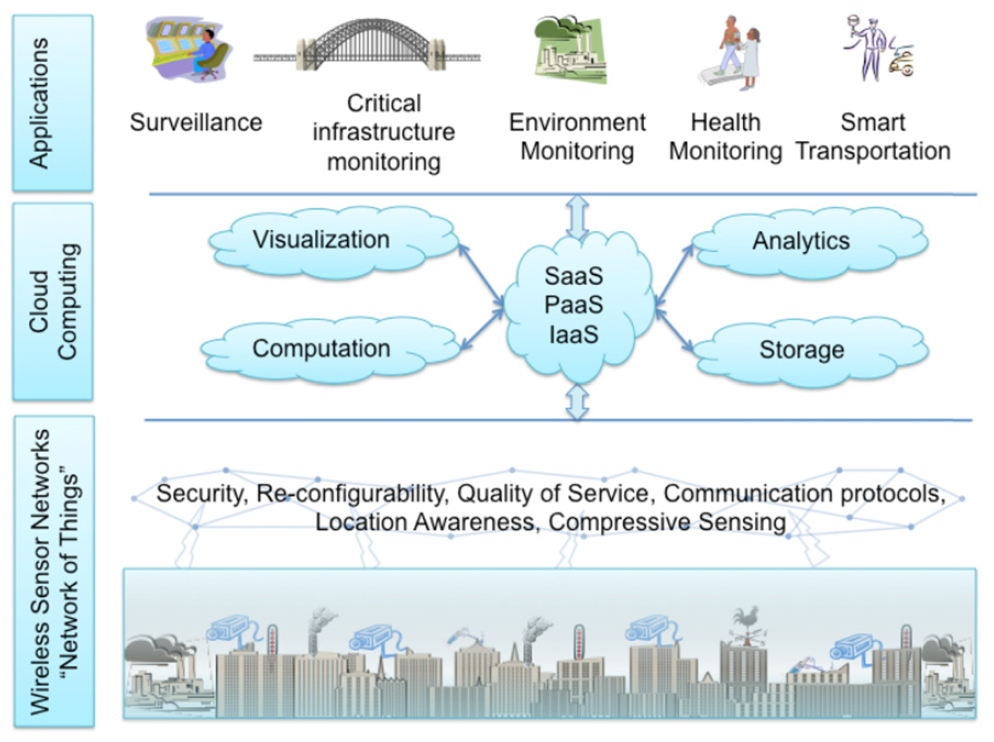
\includegraphics[width=\textwidth]{images/gubbi-iot-framework.png}
    \caption[Conceptual framework for IoT applications]{A conceptual framework for \gls{IoT} applications, integrating the world of `things' (in \glspl{WSN}) with the digital world of the Internet. \cite{gubbi-iot-vision}}
    \label{fig:intro:iot:framework}
\end{figure}

In order to integrate such a large number of devices into the global Internet infrastructure, \gls{IoT} devices use \gls{IPv6} for networking. The \gls{IPv6} address space allows for $2^{128}$ possible addresses, which is more than plenty to support the rapid growth of these devices. The same technologies that power the Internet are adapted to the scale of \gls{IoT} devices, such that they can communicate with outside networks in a uniform and transparent manner. For example, \gls{IoT} devices can send and receive \gls{IPv6} packets, download a file from a website, or even host a small web server.

The (possible) applications for \gls{IoT} encompass nearly all fields, ranging from improving comfort at your own house to controlling critical wide-range infrastructures:
\begin{description}
\item[Smart homes.] By connecting household appliances, temperature sensors and security cameras to the Internet, a house owner could control his living comfort from any device at any time \cite{chan-smart-home-review}. Instead of having to deal with many different switches and remotes around his house, he could have a single dashboard to monitor and control all of his devices. Such a dashboard could also allow for combined actions with multiple devices, for example activating the air conditioning also automatically closes the window blinds and the room doors.
\item[Smart energy grids.] With the shift from fossil resources to renewable resources, energy production is becoming more volatile and less predictable. Whereas coal and nuclear power plants can produce electricity at any time, the energy output of solar and wind plants depends on the time and weather conditions. This can lead to shortages or blackouts during calm cloudy days, or oversupply on windy sunny days. To deal with these fluctuations, smart energy grids should have the capability of predicting consumption behaviour on a more fine-grained basis, and shifting consumption peaks to better match production capacity  \cite{gungor-smart-grid-survey}. For example, houses could be fitted with smart meters which continuously measure electricity consumption and report frequently to the energy producers so they can make better predictions. Smart washing machines could also be programmed to activate when the energy demand is low, in order to shift consumption peaks. These meters and appliances need to communicate with each other and with the rest of the energy grid, posing many \gls{IT} challenges for the supporting \gls{IT} architectures and technologies \cite{gungor-smart-grid-technologies}, shown in figure \ref{fig:intro:iot:smart-grid}.
\item[Earthquake and volcano monitoring.] To protect people living in seismically active regions such as fault lines and volcanoes, scientists must be able to predict future earthquakes or eruptions so people can be evacuated in time. Improving these predictions requires more frequent and accurate seismic measurements. However, sending humans into the field to measure seismic activity is dangerous. Instead, a network of monitoring devices can be deployed to collect measurements and report back to a base station \cite{reventador} (illustrated in figure \ref{fig:intro:iot:reventador}). These devices can make more frequent measurements, and can be deployed in more dangerous places where it is unsafe for humans (e.g. inside the crater of a volcano).
\end{description}

\begin{figure}
    \centering
    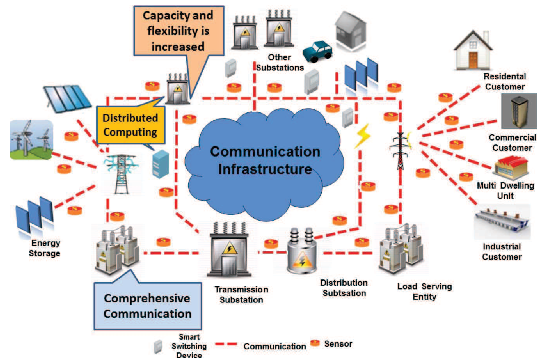
\includegraphics[width=\textwidth]{images/smart-grid-architecture.pdf}
    \caption[Example of a smart energy grid architecture]{A smart energy grid architecture. \cite{gungor-smart-grid-technologies}}
    \label{fig:intro:iot:smart-grid}
\end{figure}

\begin{figure}
    \centering
    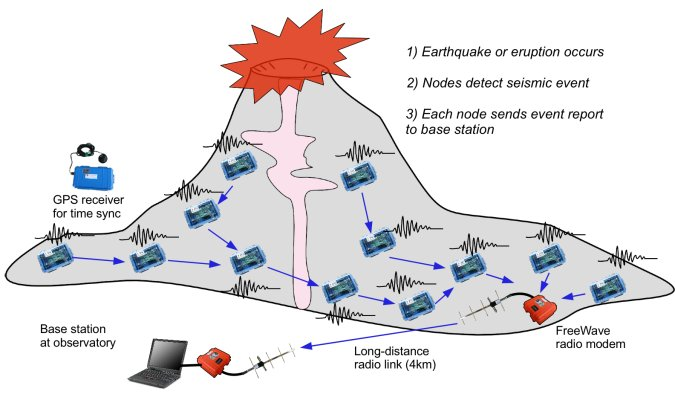
\includegraphics[width=\textwidth]{images/reventador.jpg}
    \caption[Example of IoT deployed on active volcano]{An \gls{IoT} deployed by the Harvard Sensor Networks Lab on an active volcano to monitor seismic activity. \cite{reventador}}
    \label{fig:intro:iot:reventador}
\end{figure}

\subsection{Wireless sensor networks}
\label{sec:intro:wsn}
Many \gls{IoT} applications are implemented using a \acrfull{WSN}. A \gls{WSN} consists of a number of small devices (often called `nodes' or `motes') equipped with sensors, actuators and a wireless antenna. These nodes measure changes in their environment using their sensors, communicate with each other and the outside world using their wireless connectivity and act upon their environment using their actuators.

These nodes have very different characteristics compared to regular computers, and have different design concerns for their programs:
\begin{itemize}
\item Due to their small size, they have extreme resource constraints. Whereas ordinary computers have multi-core \gls{GHz} processors with many \glspl{GB} of RAM, \gls{WSN} nodes have single-core \gls{MHz} microprocessors with only a few \glspl{KB} of RAM. For example, the tiny TMote Sky has a 8 \gls{MHz} microprocessor with 48 \gls{KB} of \gls{RAM} \cite{tmote-sky-manual}, while the larger AVR Zigduino r2 platform runs at 16 \gls{MHz} with 128 \gls{KB} of flash \gls{RAM} \cite{zigduino-manual}.
\item When deployed in remote outside locations (e.g. on a volcano or along a river), they have to be battery-powered or self-provisioning (e.g. small solar panel). This makes energy consumption a primary design concern for programmers, as the node's lifetime is constrained by its battery.
\item Nodes have no infrastructural support: there are no routers or wireless access points to support their communication. All nodes are responsible for sensing their environment, processing their data and routing messages across the network.
\item \gls{WSN} deployments are inherently unreliable. Nodes may fail due to their batteries running out or being destroyed by the environment (e.g. floods, fires or earthquakes). Transmitted messages may be lost due to bad weather conditions. Programmers must design with these failures in mind.
\item \glspl{WSN} are highly distributed. A network may consist of hundreds or thousands of nodes, with nodes moving in and out of range of each other all the time. Distributed programs must be able to scale up to large number of nodes and remain efficient.
\item A single \gls{WSN} may consist of many different types of devices with varying capabilities, specifications and architectures. Programs need to be compiled and configured to work on different device types.
\end{itemize}

\begin{figure}
	\centering
	\begin{subfigure}[b]{.5\textwidth}
		\centering
		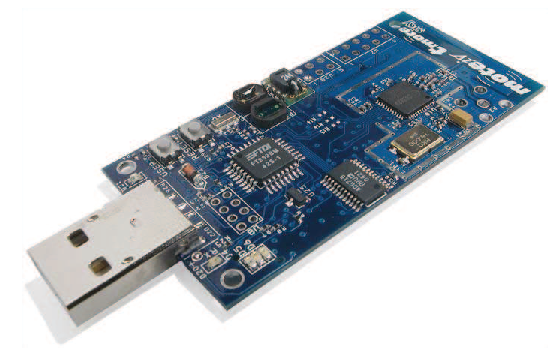
\includegraphics[width=\textwidth]{images/tmote-sky.pdf}
		\caption{The TMote Sky platform.}
		\label{fig:intro:motes:sky}
	\end{subfigure}%
	\begin{subfigure}[b]{.5\textwidth}
		\centering
		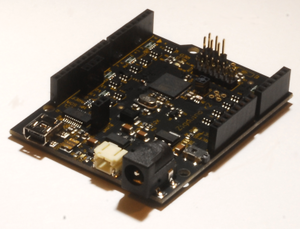
\includegraphics[width=\textwidth]{images/zigduino-r2.png}
		\caption{The AVR Zigduino r2 platform.}
		\label{fig:intro:motes:zigduino}
	\end{subfigure}
	\caption{Sample platforms for WSN motes.}
	\label{fig:intro:motes}
\end{figure}

In order to support wireless \gls{IPv6} connectivity for these low-powered devices, new Internet standards were introduced:
\begin{itemize}
\item \gls{IEEE} 802.15.4 \cite{ieee-802.15.4} specifies the physical network layer and media access control. It focuses on low power and low data rate wireless connectivity among inexpensive devices, as opposed to e.g. Wi-Fi which provides higher data rates but uses significantly more power.
\item \acrfull{6LoWPAN} \cite{rfc6282} allows \gls{IPv6} packets to be sent over \gls{IEEE} 802.15.4 networks. The standard introduces various adaptations to achieve this, such as LoWPAN encapsulation and header compression.
\end{itemize}

To allow access from outside networks, a border router is usually deployed at the edge of the network. The border router translates between \gls{6LoWPAN} packets and standard \gls{IPv6} packets and routes packets between the \gls{WSN} and the rest of the Internet.

\subsection{Peer-to-peer architectures}
\label{sec:intro:p2p}
\Acrfull{P2P} architectures consist of peers with equal capabilities and responsibilities where the work load of the application is distributed over every peer. Peers communicate with each other to retrieve information needed to perform their part of the work, and provide information to other peers to help them with their work. Although peers may different in their resource capacity and processing power, they have the same role in the architecture and can take on the same kinds of tasks.

\Gls{P2P} architectures differ from the more classical client-server architectures, in which a server \emph{provides} resources or services to be \emph{consumed} by one or more requesting clients. Clients and servers are two distinct roles in the architecture with different capabilities responsibilities, and take up distinct parts of the application's work load. For example, the client is not concerned with how the server manages its resources and services, and the server is not concerned with what the client does with the provided resource or service.

Figure \ref{fig:intro:arch} gives an overview of client-server and \gls{P2P} architectures. Figure \ref{fig:intro:arch:client-server} shows multiple clients requesting services from a single server, and figure \ref{fig:intro:arch:p2p} shows many peers communicating to request and provide services among each other. Note that clients in the client-server architecture always communicate with the server and do not communicate directly with each other, whereas peers in the \gls{P2P} architecture can communicate with any other peer.

Many Internet applications use a client-server architecture. For example, the Web consists of web servers providing web pages and web browsers requesting them. Web browsers act as clients and are responsible for sending \gls{HTTP} requests to the appropriate web server and rendering their responses as web pages on the user's screen. Web servers listen for \gls{HTTP} requests and are responsible for producing a response. The web server can do all sorts of processing behind the scenes (e.g. accessing a database) to generate this response, but the client doesn't need to know about any of this and is only concerned with the server's response.

\Acrlong{P2P} applications are less common, but have interesting applications. BitTorrent is a popular \gls{P2P} file sharing protocol, where peers download and upload parts of a file to each other to help distribute the file to all peers (see \ref{sec:related:bittorrent}). Cryptocurrencies such as Bitcoin \footnote{\url{https://bitcoin.org/}} are a fairly recent invention, where peers verify and propagate transactions of a digital currency to ensure that every peer agrees on how much money every user has -- without the need for a centralized authority such as a central bank. In both applications, every peer has the same role in the architecture and can communicate with any other peer.

\begin{figure}
	\centering
	\begin{subfigure}[b]{.5\textwidth}
		\centering
		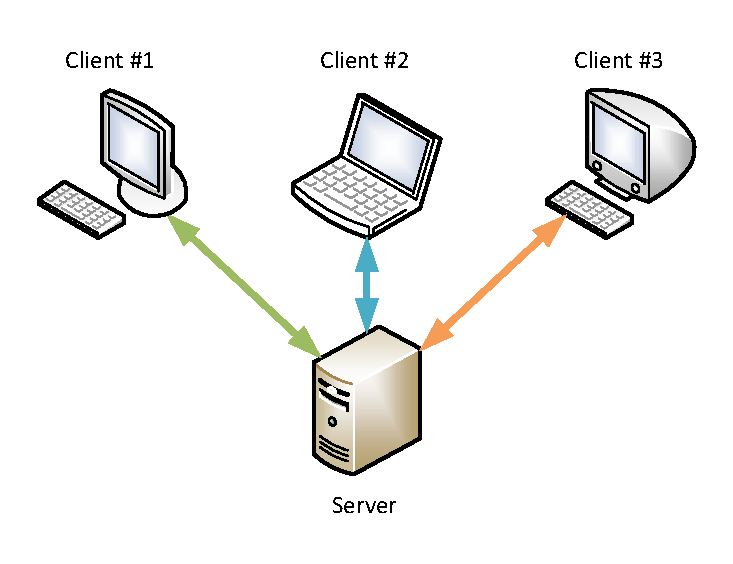
\includegraphics[width=\textwidth]{diagrams/client-server.pdf}
		\caption{Client-server architecture.}
		\label{fig:intro:arch:client-server}
	\end{subfigure}%
	\begin{subfigure}[b]{.5\textwidth}
		\centering
		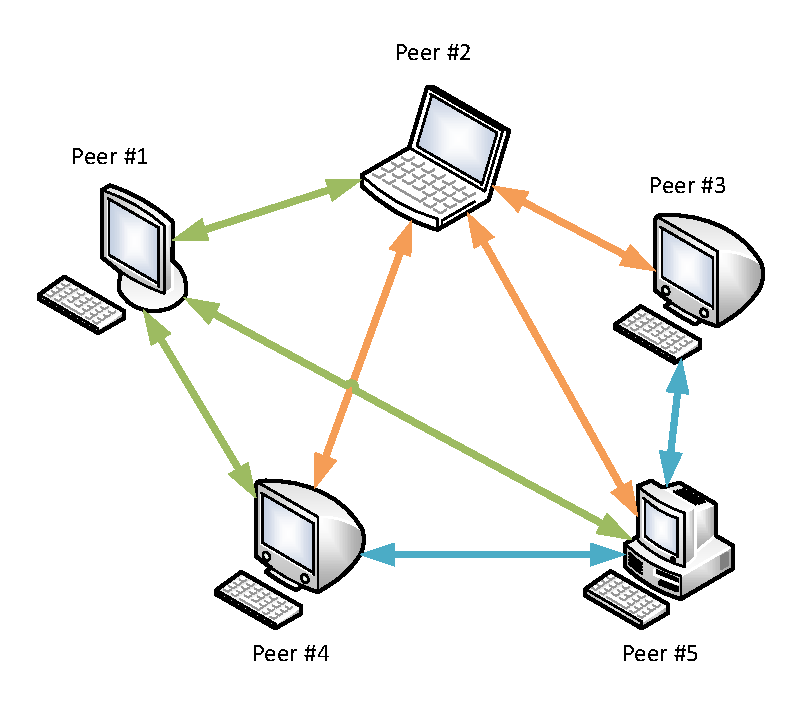
\includegraphics[width=\textwidth]{diagrams/p2p.pdf}
		\caption{Peer-to-peer architecture.}
		\label{fig:intro:arch:p2p}
	\end{subfigure}
	\caption[Server-client and P2P architectural overview]{Overview of server-client and \gls{P2P} architectures.}
	\label{fig:intro:arch}
\end{figure}

\section{Problem description}
\label{sec:intro:problem}
In order to keep \acrlongpl{WSN} operating for long periods of time, they must be able to adapt and evolve even after deployment. Over time, nodes may need to be updated with an updated program binary, a new configuration file or a new data set to be processed. However, it is often not practical and sometimes even impossible to collect a deployed node, take it back to a lab to be reprogrammed with the updated data and then re-deploy it in its original location. Therefore, these updates need to be done `over-the-air': they must be distributed over the \gls{WSN} and received by all destined nodes so these nodes can reconfigure themselves.

For such over-the-air reconfigurations, \gls{WSN} nodes need to be equipped with the proper reconfiguration mechanisms. For example, in the current version (2.0.3) of the LooCI \cite{looci} platform for Contiki \cite{contiki} nodes, the reconfiguration engine is responsible for listening for reconfiguration events, downloading the new program file over \gls{TCP} and reprogramming the node with the downloaded program. This allows LooCI nodes to be completely reprogrammed remotely, without physical intervention. However, this solution is client-server based, with all nodes requesting the download from a single server. When the number of nodes becomes larger, this can put a lot of strain on both the server and the network as many \gls{TCP} connections try to reach this single server. In contrast, a \gls{P2P} approach would balance the load over all the nodes in the network by having them all participate in the program file's distribution. This allows it to be more battery-efficient on the nodes closest to the file's source, and more scalable when the network expands.

This master's thesis focuses on the file distribution mechanism for over-the-air reconfigurations. The objective is to design, implement and evaluate a file distribution protocol optimized for \glspl{WSN}. This protocol could then be used in a complete reconfiguration solution, for example it could replace the \gls{TCP} download in LooCI, allowing for a more efficient program file distribution.

The peculiarities of \acrfullpl{WSN} (discussed in \ref{sec:intro:wsn}) pose many challenges for the design of a file distribution mechanism:
\begin{itemize}
\item File distribution requires large pieces of data to be transmitted in a short time, much larger than usually sent during normal operation of the \gls{WSN}. The transmissions sent between nodes during normal operation most of the time fits in a single packet. This data usually consists of a few measurements, a new average or a notification to the other node -- which all take up only a couple of bytes. However, large files such as programs or configurations do not fit in a single communication packet and cause much more traffic than normal operations. Since most of a node's energy is spent on its antenna and radio, a file distribution mechanism for \glspl{WSN} should be efficient with the amount of packets needed to transmit the whole file in order to save the node's battery.
\item The file should be distributed fast enough to allow nodes to return to their normal operation quickly. While a new program or configuration is propagating through the network, normal operations are largely halted. When nodes cannot be used for their intended purpose for a prolonged period of time, they might miss important measurements or fail to respond to critical events in the environment.
\item Nodes should be able to continue file distribution even when one or more nodes fail, either temporarily or indefinitely. Nodes may need to re-download (a part of) the file and/or use a different route, but a single failure must not take down the whole network. When a failed node comes back online, it should be able to resume the file distribution, preferably without having to restart the download from scratch.
\item Integrity of the distributed file must be guaranteed at every node. The file must be delivered correctly, since any error could corrupt the distributed program or configuration file. Since \glspl{WSN} are unreliable, file distribution mechanisms must be able to verify the received file and recover from transmission errors.
\item The file distribution mechanism must be able to target any subset of nodes in a \gls{WSN}. \glspl{WSN} can be heterogeneous, consisting of different kinds of nodes running different tasks. For example, a \gls{WSN} to measure weather conditions could consist of different nodes to measure temperature, humidity or wind speeds. These nodes have different sensors and run different programs, but can be part of the same network.
\end{itemize}

\section{Contributions}
\label{sec:intro:contrib}
This master's thesis presents NanoTorrent as a possible solution for file distribution in \acrlongpl{WSN}.

NanoTorrent takes a \acrlong{P2P} approach to the problem, where nodes act as peers and download and upload pieces of the file to each other. The design is inspired by the BitTorrent protocol, which has proven to be very successful on the Internet scale. By adopting ideas from BitTorrent, the solution can provide fast distribution speeds to many nodes without the need of an individual high-speed file server. However, it includes many adaptations to take advantages of the unique properties of \glspl{WSN} (discussed in \ref{sec:intro:wsn}) and deal with their challenges (mentioned in \ref{sec:intro:problem})

The main contribution of NanoTorrent is the exploration of a hybrid peer discovery mechanism. BitTorrent mainly uses a tracker for discovering peers, while existing \gls{WSN} distribution protocols only discover directly connected neighbour nodes. NanoTorrent combines both approaches into one solution, where the two mechanisms are used in parallel to connect with both close-by local peers and distant remote peers. This allows NanoTorrent to function in more heterogeneous \gls{WSN} deployments, where not all nodes run the same program or are located on different networks.

The evaluation of the protocol shows that NanoTorrent can provide fast file distribution in many different network configurations. The distribution speed scales well with the size of the network, although in its current form the amount of transmissions is still an issue. The hybrid peer discovery approach means that peers send a lot of messages to discover other peers, and can find distant peers which require messages to take multiple hops across the network to reach them. More research and experimentation is needed to reduce the needed communications.

\section{Structure of the text}
\label{sec:intro:structure}

\begin{itemize}

\item Chapter \ref{cha:intro} is an introduction to the problem context of \gls{IoT} and the challenges posed by file distribution for \glspl{WSN}. It outlines the contributions of this master's thesis.

\item Chapter \ref{cha:related-work} discusses the researched related work regarding \gls{P2P} protocols on the Internet and in \glspl{WSN}.

\item Chapter \ref{cha:discovery} introduces the first half of NanoTorrent's protocol design, with the hybrid peer discovery mechanism. It describes both the centralized approach with a tracker managing the swarm, and the localized approach using link-local multicast announcements.

\item Chapter \ref{cha:distribution} gives the other half of the protocol design, focusing on the file distribution aspect. It discusses the different parts of the protocol, such as how peers connect with each other, how they exchange pieces and how it takes advantage of locality.

\item Chapter \ref{cha:implementation} explains the technicalities of the create prototype implementation. It describes the system architecture and its components such as the tracker, the border router and the peers.

\item Chapter \ref{cha:evaluation} discusses the evaluation of the protocol design and the prototype implementation. Experiments were performed in a simulated environment to analyse the scalability of the protocol, and its operation in a heterogeneous network.

\item Chapter \ref{cha:conclusion} concludes the text with a summary of all chapters, the lessons learned in making this thesis and possible future work building on this thesis.

\end{itemize}
\chapter{Related work}
\label{cha:related-work}
This chapter discusses the related work researched while designing the NanoTorrent protocol. Section \ref{sec:related:internet} elaborates on \acrlong{P2P} protocols for the Internet like BitTorrent, whereas section \ref{sec:related:wsn} looks at protocols designed for \glspl{WSN}. As an exploration for a potential use case, section \ref{sec:related:evolution} looks at software evolution in \glspl{WSN}. Section \ref{sec:related:discussion} concludes with a critical discussion of the researched material.

\section{Peer-to-peer distribution for the Internet}
\label{sec:related:internet}

\subsection{BitTorrent}
\label{sec:related:bittorrent}
BitTorrent \cite{bep3} is a peer-to-peer file distribution protocol designed to distribute large files to many clients over the Internet. All clients downloading the file also help uploading the file to others, helping to share the load of distributing to many clients.

BitTorrent is used to distribute operating system images (e.g. Ubuntu\footnote{\url{http://www.ubuntu.com/download/alternative-downloads}}), video game updates, free music and movies. This makes it one of the most popular file sharing protocols, accounting for 25\% of upstream traffic in North America and Europe in 2014 \cite{sandvine}.

\subsubsection{Terminology}
\begin{description}
\item[Piece] A fixed-size part of the distributed file, which can be independently distributed and verified by peers.
\item[Torrent info] The metadata describing the file to be distributed by a torrent. This consists of the file's size, the number of pieces that make up the whole file, the size of each piece and the SHA-1 hashes of all pieces. This allows a peer to verify the integrity of the entire distributed file: the peer can calculate the SHA-1 hash of each received piece and check if it matches the expected hash from the torrent info.
\item[Torrent info hash] The SHA-1 hash of the torrent info. This hash acts as an identifier for the torrent, used in messages by trackers and peers to identify the torrent. \footnote{Using a SHA-1 hash as unique identifier can (at least theoretically) cause problems due to hash collisions. However, these are usually ignored in real-life applications because they are incredibly rare. A single tracker or peer would have to handle a very, very large amount of torrents before the chance of a collision becomes realistic.}
\item[Metainfo file] A \texttt{.torrent} file used to bootstrap a BitTorrent client. This consists of the URL of the tracker to use for this torrent, and the torrent info to describe and verify the file's contents.
\item[Tracker] A server tracking the state of the swarm of one or more torrents, allowing clients to discover other peers in the swarm.
\item[Peer] A BitTorrent client participating in a torrent's distribution.
\item[Swarm] The peers of a torrent.
\item[Seed(er)] A peer which has finished downloading the entire distributed file.
\item[Leecher] A peer which are still missing parts of the distributed file.
\item[Initial seed(er)] A seed to bootstrap the torrent's distribution. This seed has not downloaded the file from other peers, but has been set up by the distributor with the entire file already available.
\end{description}

\subsubsection{Usage}
In order to share a file using BitTorrent, a distributor creates a torrent metainfo file containing details about the file to be distributed and the tracker to use. The distributor then publishes this (small) metainfo file through other channels (e.g. on a website) for users to find it. To begin distribution, the distributor sets up at least one \gls{initial-seed} to bootstrap the distribution.

To download a file using BitTorrent, a user retrieves the torrent metainfo file through some other channel (e.g. a distributor's website) and launches their BitTorrent client with this file. The client joins the swarm as a \gls{leecher} and starts downloading pieces from and uploading pieces to other discovered peers in the swarm. When all pieces are downloaded, the client becomes a \gls{seed}: it keeps uploading pieces to help other peers in the swarm.

\subsubsection{Protocol operation}
The BitTorrent protocol consists of a tracker protocol (over \gls{HTTP}) and a peer wire protocol (usually over \gls{TCP}). Figure \ref{fig:related:bittorrent} shows an overview of the architecture.

\begin{figure}
    \centering
    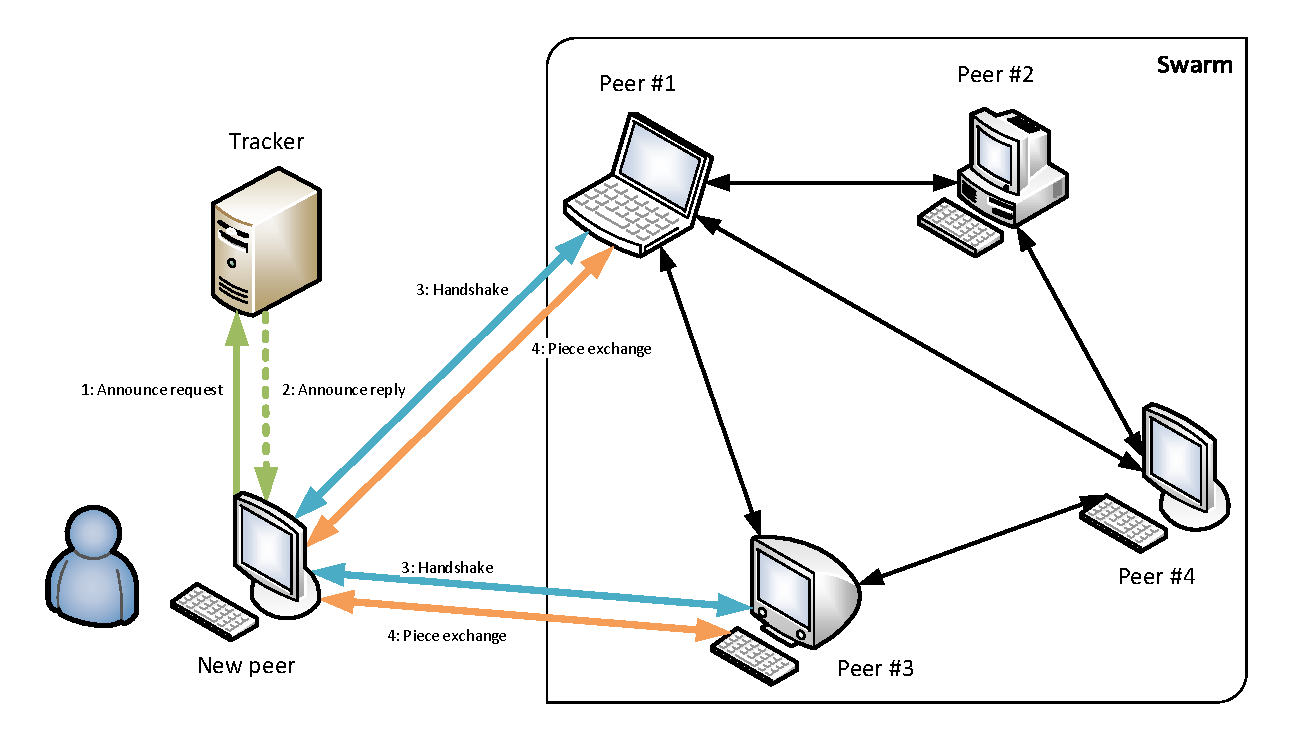
\includegraphics[width=\textwidth]{diagrams/bittorrent.pdf}
    \caption[BitTorrent architectural overview]{Overview of the BitTorrent architecture.}
    \label{fig:related:bittorrent}
\end{figure}

The client joins the swarm by sending an \emph{announce request} to the announce URL mentioned in the torrent metainfo file. The tracker receives this request, stores the new client's connection details and responds with an \emph{announce reply} containing a list of other peers with whom to connect. When other peers join the swarm, these stored connection details can be returned in their announce replies, inviting the new peers to connect with this client.

After retrieving a list of peers, the client opens \gls{TCP} connections with these peers. They both send a handshake message to ensure that both ends are indeed operating on the BitTorrent protocol and are trying to download the same torrent (identified by the metainfo hash).

After the handshake, the peers can start sending peer wire messages over the connection. The \texttt{have} and \texttt{bitfield} messages are used to notify about which pieces this peer has completely downloaded, so the other peer can potentially request them. The \texttt{request}, \texttt{piece} and \texttt{cancel} messages are used to transfer data of a single piece. This set of protocol messages is already sufficient to implement the file transfer. When a client has fully downloaded a piece, it sends a \texttt{have} message to all other peers so they are made aware of the newly available piece and may later \texttt{request} it. This continues until the client has downloaded every piece, at which point the client becomes a seed: there's nothing left to download, but it keeps uploading to help other peers in the swarm.

However, BitTorrent must also deal with limited network conditions and potentially `rogue' implementations of the protocol. \gls{TCP}'s congestion control performs poorly when sending over many connections at once, so not all opened connections should be used at the same time. Also, a `selfish' client implementation could ignore all received \texttt{request} messages, and only download from others without helping others by uploading to them. Therefore, BitTorrent clients maintain extra flags for every peer: the \emph{choke} flag means that the other end is not allowed to request data, and the \emph{interested} flag means that the other end would like to request data from this client. A peer sends \texttt{choke} or \texttt{unchoke} messages to notify whether this peer is choking the other end, and \texttt{interested} or \texttt{uninterested} messages to notify whether this peer is interested in one of the other's pieces. Clients can then use a choking algorithm to control which peers are allowed to download (by `unchoking' them), and which peers should be (temporarily) blocked (by `choking` them). For example, clients can keep only a limited number of connections unchoked, to prevent congestion. To promote `good behaviour' for clients, most BitTorrent implementations uses a \emph{tit-for-tat strategy} for their choking algorithm. With this strategy, peers will choke the other end when they are being choked (hence tit-for-tat), and will try to unchoke the other end when they are unchoked and the other end is interested.

\subsubsection{Advantages and disadvantages}
Every peer downloading missing pieces of the torrent's file also uploads the pieces it already has to other interested peers. This peer-to-peer file sharing approach has many advantages for both clients and distributors:
\begin{itemize}
\item Instead of having a single file server serving all clients wanting to download the file, BitTorrent employs the (often underused) upload capacity of those clients to help distributing the file to other clients. The combined upload capacity of these clients can be very large, and comes almost free to the distributor. The distributor only has to invest in a modest server acting as an initial seed, and letting the clients share the load.
\item Clients can download many pieces from many peers in parallel, which can lead to faster downloads.
\item BitTorrent is more failure-resilient than regular file distribution protocols such as \gls{FTP}. The \gls{FTP} server is a single point of failure: nobody can download the file if the server fails. In contrast, the failure of a single BitTorrent peer does not greatly impact the rest of the swarm. If every piece owned by the failed peer is still available at some other peer, all remaining peers can still download the full file. When the failed peer restarts, it also doesn't need to restart the complete download: it can verify the previously downloaded pieces using the checksums and resume downloading the missing pieces.
\item Regular file distribution protocols do not scale well when the number of simultaneously connected clients increases. \gls{FTP} requires 2 \gls{TCP} connections for each connected client trying to download a file, which can quickly consume the server's resources. The server also uses more upload bandwidth, which can cause congestion in the network. The classic solution to this involves installing more servers (`mirrors') in more locations, but this is expensive. In contrast, the load on the initial seed in BitTorrent actually \emph{decreases} as a torrent becomes more popular: all connected clients share the load to help others download the file.
\end{itemize}

However, there are also disadvantages to moving to peer-to-peer distribution:
\begin{itemize}
\item Unpopular torrents can become abandoned, with no active seeds in the swarm. This means that no new peers can download the full file, rendering the torrent useless until a seed is re-introduced. To prevent this, the distributor should maintain at least one seed in the torrent. This ensures that in the worst-case scenario, the whole file can be retrieved from the distributor's seed.
\item Moving the upload load from the distributor to the clients means that the networks of clients see more upload traffic. \glspl{ISP} optimize their consumer networks for `regular' consumer traffic behaviours, which consists primarily of download traffic. An \gls{ISP} might throttle torrent traffic in order to `shape' the traffic to a desired profile, reducing the performance of BitTorrent peers on its network.
\end{itemize}

\subsection{Local Peer Discovery for BitTorrent}
\label{sec:related:bt-ldp}
Local Peer Discovery is a BitTorrent protocol extension designed to support the local discovery of peers, aiming to maximize torrent traffic through the \gls{LAN} and reduce traffic through the \gls{ISP} \cite{bt-ldp}. Although there is no formal specification published as of the time of writing \footnote{Due to this lack of published specification, the only decent source \cite{bt-ldp} is on Wikipedia.}, it is quite consistently implemented in various BitTorrent clients and supports both \acrshort{IPv4} and \acrshort{IPv6} multicast.

The extension introduces a new discovery mechanism parallel to the centralized tracker, which uses \gls{UDP} messages periodically sent to a local multicast address to announce and discover peers in the local network. These messages are similar to standard announce requests, and include the torrent info hash and peer connection details. When other peers in the \gls{LAN} receive this multicast message, they can read the connection details and try to establish a peer connection.

Local Peer Discovery is not used very often in practice, as home user \glspl{LAN} are small and it is fairly uncommon to have many users downloading the same torrent inside the same local network. It makes much more sense in \glspl{WSN} where many peers do share the same local network, which is why this peer discovery mechanism is included in the protocol design (see \ref{sec:discovery:local}).

\section{Peer-to-peer distribution for WSNs}
\label{sec:related:wsn}

\subsection{Deluge}
\label{sec:related:deluge}
Deluge \cite{deluge} is a reliable data dissemination protocol for propagating large data objects from one or more source nodes to many other nodes in a \gls{WSN}. It allows incremental updates of large files to be efficiently flooded to the whole network.

Deluge assigns a monotonically increasing \emph{version number} to each new version of the distributed object, and subdivides the object into fixed-size pages. Since new versions often only have small difference compared to the previous version, many pages do not change between versions. Deluge uses this information to re-use pages from previous versions and prevent redundant page transfers. Every new page is identified by a monotonically increasing \emph{page number}.

Deluge nodes send periodic local broadcasts announcing their current version number and the latest available page (with the guarantee that all previous pages are also available). To control the transmission of potentially redundant announcements, Deluge uses the Trickle algorithm \cite{trickle} to do a `polite gossip'. For example, when a node hears a lot of its neighbours announcing the same version that it already has, it knows that there's no point in announcing its own version again. Most of its neighbours will probably already have heard one of the other neighbour's messages, so the node stays quiet to avoid broadcasting a redundant message.

\begin{figure}
    \centering
    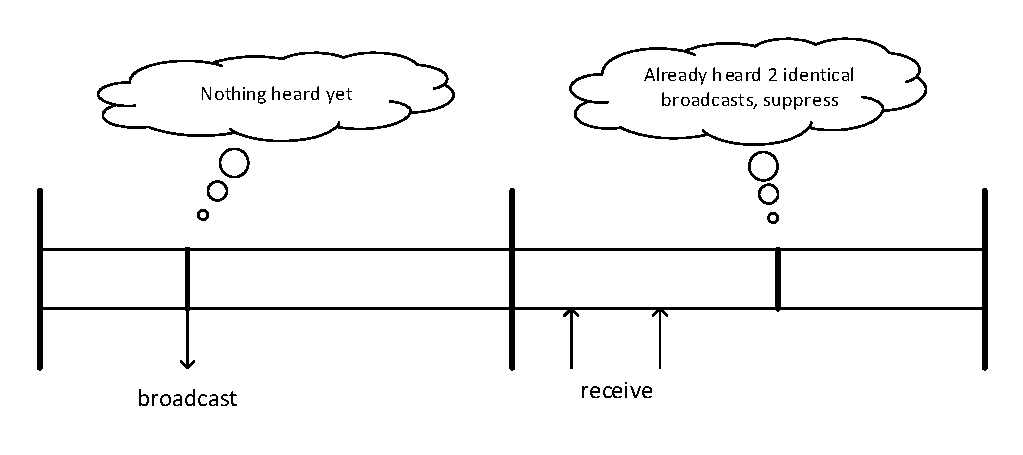
\includegraphics[width=\textwidth]{diagrams/trickle.pdf}
    \caption[Trickle algorithm example]{Example of Trickle's polite gossip algorithm. In the first interval, the node hasn't heard any other broadcasts yet and sends its broadcast. In the second interval, two identical broadcasts have already been received before the own broadcast is due, therefore the node suppresses its redundant broadcast.}
    \label{fig:related:trickle}
\end{figure}

Figure \ref{fig:related:trickle} shows an example of the Trickle algorithm in action. Before every interval, the node picks a random time $t \in [0, \tau]$ at which to schedule its own broadcast. If it doesn't hear a certain number of other identical broadcasts, it will send its broadcast at time $t$. If it does receive enough identical broadcasts, it will suppress its own broadcast at time $t$ and will not send anything during this interval. Because $t$ is randomly re-generated after every interval, the cost of sending broadcasts is distributed among all neighbours, ensuring that nodes use on average the same amount of energy for maintaining the announcements.

When a node hears one of its neighbours announcing a newer version number, it must update to the new version. Since many of its neighbours will hear this same announcement and likely also need to update, it would be wasteful for all these nodes to send requests to retrieve the new pages. Once again, Trickle is used to prevent redundant messages, so only a couple of nodes will send a broadcast to request the new page and only a few nodes will reply to the request. This allows new pages to propagate very efficiently throughout the network.

Deluge takes great advantage of local broadcasts in \glspl{WSN}, and makes flooding code updates very efficient. However, it assumes that all nodes in the network all need the same file, which might not be the case in heterogeneous deployments. NanoTorrent takes some advantage of local broadcasts by sending piece data as local multicasts (see \ref{sec:distrib:multicast}), however it can also use unicast messages to reach distant peers in a heterogeneous network.

\subsection{TinyTorrents}
\label{sec:related:tinytorrents}
TinyTorrents \cite{tinytorrents} is a peer-to-peer protocol designed for data dissemination in \glspl{WSN}. Like BitTorrent, TinyTorrents uses torrent files to describe the tracker's location and the file's contents. Peers join the swarm by contacting the tracker, and discover other peers with whom to connect and exchange data.

TinyTorrents recognizes that many of the problems BitTorrent tries to solve on the Internet also match the challenges posed by \glspl{WSN}. BitTorrent balances traffic load with its \gls{P2P} approach and avoids network partitions with a tracker. Data integrity is ensured with piece-wise checksums, and data replication is made efficient with its rarest-first piece selection policy. TinyTorrents adopts these design decisions, and similarly NanoTorrent follows the same reasoning.

However, BitTorrent's peer wire protocol consists of many short frequent messages such as \texttt{have}, \texttt{choke} and \texttt{interested} (explained in \ref{sec:related:bittorrent}). These are decremental for \gls{WSN} nodes, as they consume a lot of energy for transmission. TinyTorrents solves this by combining separate \texttt{have} messages into one less frequently sent \texttt{bitfield} message, and using a static approach based on the peer's position in the swarm to fairly distribute the load among \glspl{seeder} and \glspl{leecher}. NanoTorrent also drops BitTorrent's short \texttt{have} messages, but its tracker does not currently take fairness into account.

TinyTorrents supports interoperability with standard BitTorrent through a gateway acting as a bridge between the two protocols. The gateway can convert TinyTorrent torrents into BitTorrent torrents, allowing regular BitTorrent clients to download data from inside the \gls{WSN} and allowing \gls{WSN} nodes to download torrents published outside the \gls{WSN}. This allows remote users to access accumulated sensor measurements from the \gls{WSN}, or to reprogram nodes from anywhere on the Internet. NanoTorrent does not currently interoperate with BitTorrent, but can support interoperation with nodes on other \glspl{WSN} or the Internet thanks to its \gls{IPv6} foundation.

The authors of TinyTorrents recognize that their reliance on a centralized tracker is a weak point of their protocol, which is a single point of failure in their system. NanoTracker attempts to alleviate this by combining multiple peer discovery mechanisms, so peers can still discover each other even if the tracker (temporarily) becomes unavailable.

\section{Software evolution in WSNs}
\label{sec:related:evolution}

\subsection{Challenges and approaches for reprogramming WSNs}
Wang et al. \cite{wang-reprogramming} outline a framework to examine the different functions for a reprogramming solution for \glspl{WSN}, and survey the approaches taken by existing solutions.

Figure \ref{fig:related:wang-framework} shows their framework for reprogramming solutions. This includes features such as version control to manage different software versions, scope selection to control which nodes are affected by a reprogramming operation and code acquisition to request the download of a new version.

The authors note that \glspl{WSN} come with many challenges. The algorithms used on a \gls{WSN} node must be well designed to fit the constrained capacity profile of the node, they must be scalable and energy-efficient, and they must be able to handle unreliable communications.

The paper groups the approaches of various existing code dissemination protocols like Deluge by categories, such as the scope of an individual reprogramming operation, the ability to traverse a multi-hop network and the use of pipelining to accelerate the distribution. Although many protocols support multi-hop reprogramming, only a few such as Aqueduct and TinyCubus have support for a limited scope reprogramming.

Important objectives for a good reprogramming solution are reliability, scope coverage and autonomy: all targeted nodes must be able to autonomously and correctly retrieve the new software version. For practical usefulness, it must also be fast enough to cause minimal disruption to the normal operation of the \gls{WSN}, consume only a minimal amount of energy during the transmission and use only a minimal amount of \gls{RAM}.

In their framework, a \gls{P2P} file distribution protocol for \glspl{WSN} could fulfil the code acquisition and code dissemination functions of a network reprogramming solution. When a peer finds out that it should update to a new version, it can connect with the other peers with that same version and start exchanging the file with them.

\begin{figure}
    \centering
    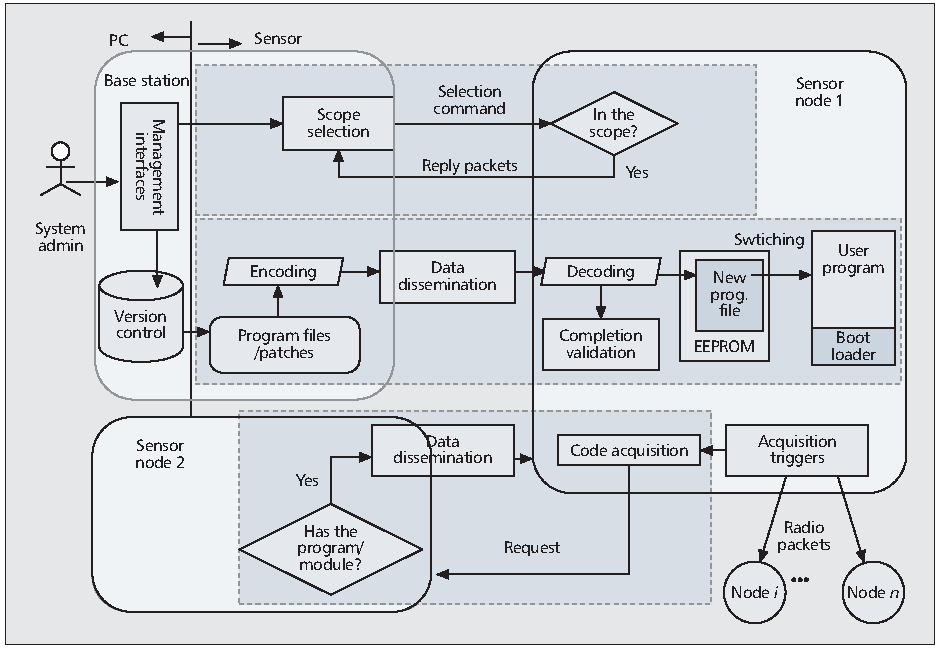
\includegraphics[width=\textwidth]{images/wang-reprogramming-framework.pdf}
    \caption[Framework for WSN reprogramming solutions]{Framework for WSN reprogramming solutions. \cite{wang-reprogramming}}
    \label{fig:related:wang-framework}
\end{figure}

\section{Critical discussion}
\label{sec:related:discussion}
BitTorrent has shown that \gls{P2P} file distribution can be made fast and easy-to-use on the Internet. It introduced a lot of good ideas, such as the choke/interested flags to control network load and punish misbehaving peers with a tit-for-that algorithm. However, these short frequent control messages can cause a lot of network traffic, which is the main cost factor for \gls{WSN} nodes. The design of a protocol aimed at \gls{WSN} nodes should be more careful with its transmissions.

BitTorrent Local Peer Discovery shows that multicast messages can be used to discover other peers on the same \gls{LAN} for faster local file distribution. However, multicast is not well supported in the current Internet infrastructures, many of which still use \gls{IPv4}. It is also very unlikely to have multiple BitTorrent clients on the same network downloading the same torrent, as consumer \glspl{LAN} are usually very small and corporate \glspl{LAN} mostly refrain from allowing BitTorrent traffic on their networks. This makes BitTorrent's Local Peer Discovery very underused on the Internet. However, the ideas behind its design are sound, and can be useful in the context of \glspl{WSN}.

There exist already a number of \gls{P2P} file transfer protocols for \glspl{WSN}. Deluge uses local broadcasts and listens for other neighbour's messages to prevent redundant transmissions. TinyTorrents is also influenced by BitTorrent's design, and even provides interopability with the original prototocol through the use of a gateway. However, none of these protocols leverage the \gls{IPv6} architecture which is becoming more common in \glspl{WSN} deployments as base for their communication. Deluge uses lower-level broadcasts for its communications, while TinyTorrents uses a custom TinyHop routing protocol. This opens an opportunity for a file distribution protocol which can run on top of the \gls{IPv6} network stack, allowing multi-hop connectivity between distant nodes in the network and even communication with outside networks.

A \gls{P2P} file distribution protocol for \glspl{WSN} could fulfil the code acquisition and code dissemination functions of a network reprogramming solution in the framework of Wang et al. \cite{wang-reprogramming}. Their paper also investigates protocols such as Trickle and Deluge, and notes that they only allow for full network reprogramming. There is an opportunity for a file distribution protocol that allows reprogramming of a limited scope of nodes, possibly with multiple reprogramming operations operating in parallel targeting different groups of nodes.

\chapter{Peer discovery}
\label{cha:discovery}
This chapter discusses the design of the peer discovery mechanisms in NanoTorrent. These mechanisms enable peers to discover other peers downloading the same torrent, allowing them to connect with each other and exchange file data. NanoTorrent uses a hybrid approach consisting of two peer discovery mechanisms running side-by-side, allowing it to exploit locality while at the same time keeping distant nodes connected.

Section \ref{sec:discovery:tracker} describes the client-server approach using a centralized tracker. Section \ref{sec:discovery:local} discusses the local peer discovery mechanism using \gls{IPv6} local multicasts. Finally, section \ref{sec:discovery:conclusion} concludes with a discussion of the hybrid approach.

\section{Peer discovery with centralized tracker}
\label{sec:discovery:tracker}
One approach to implementing peer discovery is using a client-server architecture where membership information is provided by a central server known as the \emph{\gls{tracker}}. This tracker maintains the state of all peers in the \gls{swarm}, and peers can discover and be discovered by other peers by sending requests to obtain (parts of) this information.

\subsection{Requirements}
The \gls{tracker} is responsible for maintaining the \emph{\gls{swarm}} of each of its torrents, i.e. the list of \glspl{peer} for every tracked torrent. It must be notified when a peer wants to join the swarm to start downloading a torrent, and when it wants to leave after it finishes downloading and seeding the torrent. In order to deal with possible peer failures, messages from peers to the tracker are also treated as a `heartbeat' for that peer. The tracker keeps track of the timestamp of the last message from each peer and periodically removes peers who have not contacted the tracker for a long time. This helps to ensure that peers will discover active peers most of the time and will not try to connect with unreachable stale peers.

Peers should be able to discover other peers by contacting the tracker and receiving a list of other peers with whom to connect. Each peer is responsible for keeping the tracker up-to-date on its own participation state, such as when it joins or leaves the swarm. This allows the peer to be discovered by other peers when they contact the tracker themselves. In order to keep their heartbeat alive at the tracker, peers need to periodically contact the tracker to refresh their state as long as they're participating in the swarm.

\subsection{Torrent descriptor}
\label{sec:discovery:torrent-desc}
Before a file can be distributed to a set of nodes in the network, these nodes must have enough information to download and verify the whole file on their own. This information is contained in a \emph{\gls{torrent-desc}} which is generated upfront and needs to be made available at every node to start the file transfer.

The \gls{torrent-desc} is similar to the \emph{metainfo} in BitTorrent, but uses a denser structure than BitTorrent. This allows for a shorter descriptor file compared to BitTorrent's \texttt{.torrent} file, and faster parsing by nodes.

A \gls{torrent-desc} consists of the \gls{IP} address and port of the tracker, and the \gls{torrent-info} (further explained in \ref{sec:distrib:piece}. Like BitTorrent, trackers and nodes use the \gls{torrent-info-hash} calculated from the \gls{torrent-info} as an identifier for a torrent (see \ref{sec:related:bittorrent}). This way, a node only needs the torrent descriptor to locate the tracker and join the swarm corresponding to the correct torrent.

The distributor must generate the torrent descriptor and make it available to all destined nodes before starting file distribution. How the torrent descriptor is made available at a node, is out of the scope of the protocol.

\subsection{Protocol}
Peers communicate with the tracker through a request-reply protocol, (unimaginatively) named NanoTracker. This is a simple request/reply protocol over \gls{UDP}, where peers send an \emph{announce request} to the tracker, and the tracker responds with an \emph{announce reply}. Since the tracker can potentially track multiple swarms for multiple torrents, every message also includes the info hash of the torrent to identify the swarm. In theory, this allows a peer to join multiple swarms and download multiple torrents concurrently, although the current implementation supports only one concurrent torrent download.

The address of the tracker is included in the torrent descriptor, which must be available to every peer to participate in the torrent. A peer sends an announce request to this address over \gls{UDP}, including the event of the request and the maximum number of peers that it wants to receive in the reply. Since different clients may have different resource constraints, a client may want to request more peers from the tracker if it wants to connect with more peers simultaneously. The event indicates the reason for sending the request, and determines how the tracker should react to the request:
\begin{description}
\item[started] The peer wants to start downloading the torrent. The tracker should add the peer to the swarm, and allow it to be discovered by other peers.
\item[stopped] The peer has stopped downloading the torrent. The tracker should remove the peer to the swarm, so it will no longer be discoverable by other peers.
\item[refresh] The peer wants to refresh its participation in the swarm. The tracker should update the peer's heartbeat timestamp, ensuring that it stays discoverable for the near future.
\item[completed] The peer has finished downloading the torrent and is now seeding the torrent. The tracker could use this information for statistics, or for prioritizing the peer in the replies for other peers.
\end{description}

The tracker selects a number of other peers from the swarm, making sure it does not exceed the maximum number of peers requested by the peer. The tracker then constructs and sends back an announce reply, which contains a list of \gls{IPv6} addresses of the selected peers. The peer stores these addresses and can then start connecting and exchanging pieces with those peers as described in chapter \ref{cha:distribution}.

\subsection{Comparison with BitTorrent}
The design of the tracker protocol is heavily inspired by the \gls{UDP} Tracker protocol for BitTorrent \cite{bep15}, but is adapted to the needs of \glspl{WSN}.

\subsubsection{IP spoofing prevention}
BitTorrent tries to prevent peers from `spoofing' their \gls{IP} addresses, i.e. using a different address as the \gls{UDP} source address than their own. A malicious user could abuse the peers in a very popular torrent's swarm for a \gls{DDoS} by spoofing an announce request with the victim's IP address. Since the BitTorrent tracker stores the source \gls{IP} address of the announce request and announces it to other peers looking to discover peers in the swarm, these peers can be tricked into sending traffic to the uninterested victim.

To prevent \gls{IP} spoofing, a peer has to first send a connect request and receive a connection identifier in the tracker's connect reply. This identifier must then be passed in every announce request and validated by the tracker. This way, the peer has to `prove' it is using its own IP address by presenting information sent to the provided source address.

In the context of \glspl{WSN}, \gls{IP} spoofing is not really a concern. Therefore, there is no need for an initial connect request/reply step and peers can immediately send announce requests.

\subsubsection{Random peer ports}
In BitTorrent, peers choose a random \gls{TCP} port to listen for incoming connections from other peers for the peer-to-peer protocol \cite{bep3}. This allows multiple torrent downloads to run on different ports without interfering with each other. However, this also means that other peers need to know both the \gls{IP} address as well as the port number of a peer in order to set up a connection. Therefore, a peer includes its port number in the announce request, the tracker stores this port along with the rest of the peer's information and announce replies contain both the IP address and the port number for each peer.

For \glspl{WSN}, it is more convenient if all peers use a fixed port number for peer-to-peer communication. This allows local peer discovery (detailed in \ref{sec:discovery:local}) to use a single multicast address and a single port to reach all local peers. A disadvantage of this approach is that now all peer messages must include the torrent's info hash to identify the torrent, as the same port could be used by multiple torrents being downloaded by different nodes in the network.

\subsubsection{Download and upload statistics}
In BitTorrent, peers must provide information about the amount of bytes they have uploaded and downloaded, as well as how much data they still have left to download in order to complete the torrent download. This statistical information can be used by the tracker for example to implement more sophisticated peer selection algorithms for generating announce replies, to analyse the `health' of the torrent or simply to display on the tracker's website.

In the context of \glspl{WSN}, this information is not really needed and therefore not supported by the NanoTracker protocol.

\subsection{Conclusion}
By centralizing membership information at a single tracker, it becomes easier to analyse the state of the swarm. An operator of the \gls{WSN} can query the tracker at any time and retrieve information about which peers are currently connected. The tracker can detect when a peer stops sending periodic announce refreshes, and notify the operator of a potentially failed peer.

However, the need to periodically refresh the swarm membership state of every peer inevitably leads to additional network traffic. It could also create a bottleneck in the section of the network closest to the tracker, where all messages from all peers in the \gls{WSN} need to pass.

\section{Peer discovery with local multicast}
\label{sec:discovery:local}
In many \glspl{WSN}, nodes with similar tasks are often deployed closely together. Some networks consist of small clusters of similar nodes, or only consist of one node type altogether. In these deployments, peers need the same files as their immediate local neighbours, and can distribute files more efficiently through local broadcasts to all of their neighbours (see \ref{sec:distrib:multicast}).

To encourage peers exchanging pieces of the distributed file with their immediate neighbours, peers need to be able to discover neighbour nodes which are downloading the same torrent. The local peer discovery mechanism achieves this by periodically sending an announcement as a multicast to all immediate neighbours. If a peer receives such a local advertisement, it can try to connect with the originating peer.

\subsection{IPv6 link-local multicast}
\gls{IPv6} supports three addressing modes: unicast, anycast and multicast \cite{rfc4291}. A unicast address identifies a single \gls{IPv6} interface, and a packet sent to it is delivered only to that interface. An anycast address identifies one or more interfaces, but a packet sent to it is delivered to \emph{one} of those interfaces. A multicast address also identifies multiple interfaces, but packets are delivered to \emph{all} of those interfaces. This is a big improvement over \gls{IPv4}, which only defines unicast and broadcast addresses (with \emph{optional} multicast support).

Orthogonal to addressing modes are address scopes, which indicate in which part of the network a given address is valid. Global addresses are valid over the whole Internet, whereas link-local addresses are only valid in a single network.

\gls{IPv6} reserves some special multicast addresses to send messages to certain types of nodes in an address scope. For example, a multicast address can target all nodes, all routers or all \gls{DHCP} servers on the same link, network or organization.

\subsection{Protocol}
The local peer discovery protocol consists of periodically sending an announcement to all direct neighbours. This allows local peers listening to these announcements to discover new peers and in return set up connections with them.

For the purpose of discovering other peers in the immediate neighbourhood, NanoTorrent currently uses the \texttt{ff02::1} link-local all-nodes multicast address. This address works like a link-layer local broadcast address (e.g. the \gls{MAC} address \texttt{ff:ff:ff:ff:ff:ff}). All nodes already listen to incoming packets on this address, requiring no extra configuration.

Rather than adding another special-purpose message type for periodic announcements, NanoTorrent re-uses the \texttt{have} message which is already periodically exchanged between peers (discussed in more detail in \ref{sec:distrib:connection}). Peers use this when setting up a connection to a newly discovered peer, and to periodically inform connected peers of their download progress. Local peer discovery is implemented by also sending these periodic \texttt{have} messages to the link-local all-nodes multicast address. When a local peer receives any message from an unknown peer, it will try to set up a peer connection and (eventually) send back their own message. This reply allows the originating peer to set up its own connection with the discovered peer, resulting in a two-way connection where both peers can request pieces.

\begin{figure}
    \centering
    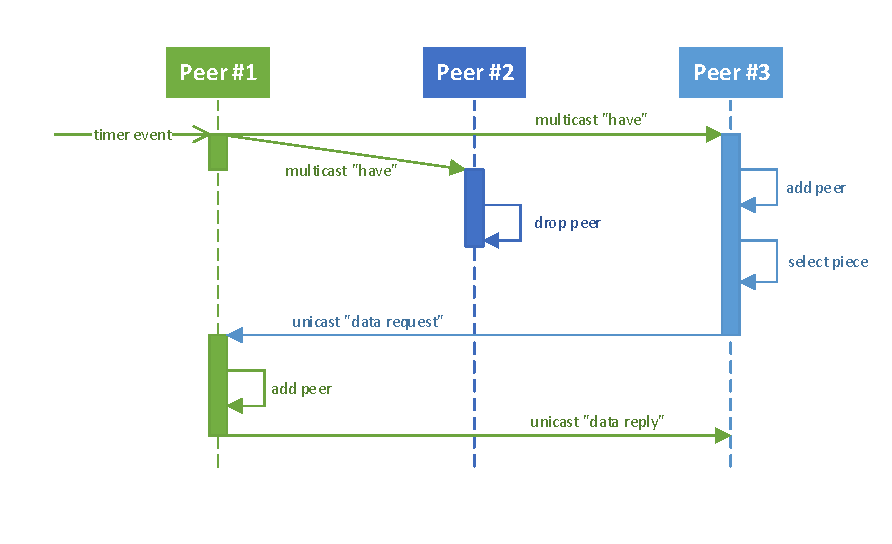
\includegraphics[width=\textwidth]{diagrams/local-peer-discovery.pdf}
    \caption[Sequence diagram of local peer discovery]{Sequence diagram of local peer discovery. The second peer has no more resources to add a connection for the first peer, and ignores the announcement. The third peer does add the new peer, and immediately requests a piece from the new peer. This allows the first peer to discover the third peer, add it and reply to the request.}
    \label{fig:discovery:local}
\end{figure}

Figure \ref{fig:discovery:local} shows a sequence diagram of a possible interaction between three neighbouring peers. The first peer sends its periodic announcement as a multicasted \texttt{have} message to all its neighbours. When they receive this message, they can choose to set up a connection with the peer if they have enough resources to do so and are downloading the same torrent. In this case, the third peer detects that the new peer has interesting pieces, and immediately sends a data request for a missing piece. The first peer receives this message from an unknown peer, which allows it to discover the third peer and add it to its own connections. It then dutifully responds to the request, and can start requesting pieces for itself. If the first peer did not have any pieces that are immediately interesting to the third peer, the third peer will later on send its own multicast announcement, so the first peer can eventually discover the third peer.

\subsection{Conclusion}
Local peer discovery can be added to NanoTorrent with minimal additional cost. For the wireless radio antenna, it doesn't matter whether a packet is destined to one or multiple nodes: all messages must be broadcasted anyway over the wireless medium. However, multicast packets do take more time for nodes to process, as they cannot short-circuit them like unicast messages. When a node receives a unicast packet destined to a different node, it can reject this as early as the link layer (using the destination \gls{MAC} address) or the network layer (using the destination \gls{IP} address). All-nodes multicast messages however always make it through to at least the transport layer, only rejecting the packet when the node is not acting as a NanoTorrent peer and therefore is not listening on the protocol's \gls{UDP} port.

By building on top of \gls{IPv6} multicast, local peer discovery can work on any \gls{IPv6}-compliant networking stack. Rather than going to a lower layer protocol such as \gls{RPL} \cite{rfc6550} for information about physical neighbours, NanoTorrent stays generic and independent of the underlying physical network infrastructure. This also allows it to re-use large parts of the existing protocol which is already designed for \gls{IPv6}.

\section{Conclusion}
\label{sec:discovery:conclusion}
Like in BitTorrent, the centralized tracker acts as a single source of (partial) truth about all active peers in a torrent's swarm. Every peer periodically announces itself to the tracker to keep its membership state alive, and in return received a list of other known peers in the swarm. Since this list is a random subset of the whole swarm, the chance of the \gls{P2P} network becoming partitioned is fairly low.

Local peer discovery ties in nicely with the peer wire protocol for the actual file distribution (see \ref{sec:distrib:connection}), and allows for a hybrid peer discovery solution. The tracker is still useful for ensuring that peers don't end up isolating themselves by only connecting to local peers, while local peers can efficiently propagate newly retrieved pieces to all of their immediate neighbours at once (see \ref{sec:distrib:multicast}).

\chapter{Peer-to-peer file distribution}
\label{cha:distribution}
This chapter discusses the design of the file distribution mechanism in NanoTorrent. These mechanisms enable peers to connect with each other, exchange download progress information and request file data.

Section \ref{sec:distrib:requirements} lists the requirements for the distribution. Section \ref{sec:distrib:piece} explains the use of fixed-size pieces to subdivide the distributed file. The management of peer connections is discussed in \ref{sec:distrib:connection}, and the actual piece exchange is described in \ref{sec:distrib:exchange}. The local peer discovery mechanism described in \ref{sec:discovery:local} allows for an optimization in the piece exchange, which is discussed in \ref{sec:distrib:multicast}. Section \ref{sec:distrib:conclusion} rounds up the chapter with a conclusion.

\section{Requirements}
\label{sec:distrib:requirements}
The distributed file must fit in the non-volatile storage of every targeted node, and thus its size is limited. Whereas files distributed on the Internet can be several \glspl{GB} in size, \gls{WSN} nodes can only store files in the orders of a couple of \glspl{KB}. For example, the \gls{EEPROM} of the AVR Zigduino r2 platform, (used in the evaluation in chapter \ref{cha:evaluation}) can hold up to 4 KB of data \cite{zigduino-manual}. The file distribution protocol is dimensioned to work well with these relatively small files, in its current form up to 64 \gls{KB} ($2^{16}$ bytes).

The protocol should attempt to prevent redundant communications. For examples, peers should not request parts of the files from another peer if they do not know whether the other peer already has that part available. Therefore, peers should advertise information about their own download progress to others so they can make informed requests. This implies that peers need to retain stateful information about other peers.

Peers should try to balance the overall load on the \gls{P2P} network. If a certain piece of the file were only available at one single peer (which is often the case with an \gls{initial-seed} early on in the \gls{swarm}'s lifetime), that peer could become overloaded when other peers do not properly coordinate their requests. In the worst case, a failure of that single peer could prevent the rest of the network from receiving the whole file. The protocol should try to relieve peers with highly wanted file pieces, and prioritize their distribution over more commonly available pieces.

File distribution must be robust against corruptions and transmission errors. For example, when distributing a new program binary, it is crucial for the program's correctness and stability that the received file is bit-for-bit identical to the original. Therefore, \glspl{peer} must be able to independently verify the integrity of the received file in its entirety.

\section{Pieces}
\label{sec:distrib:piece}
NanoTorrent uses the same approach as BitTorrent to subdivide the distributed file in fixed-size \emph{pieces} which can be independently distributed over the \gls{P2P} network. This allows peers to retrieve them in any order and download multiple pieces from multiple peers in parallel (see \ref{sec:related:bittorrent}).

All information about a torrent's pieces are contained in the \emph{\gls{torrent-info}}, which is part of the \gls{torrent-desc} (detailed in \ref{sec:discovery:torrent-desc}). Peers can verify the integrity of the entire file by verifying the integrity of each individual piece. The SHA-1 hash of the torrent information (further abbreviated to \emph{info hash}) is used to tag all messages exchanged between peers, to ensure that messages for different torrents do not interfere with each other.

\section{Peer connections}
\label{sec:distrib:connection}
Peers can discover other peers in two ways: they can find out about another peer through the tracker (detailed in \ref{sec:discovery:tracker}), or they receive a message from another peer (which includes local peer discovery  from \ref{sec:discovery:local}). Both give the peer an \gls{IPv6} address of another peer, which they can use to directly communicate with the peer.

However, peers need to maintain some connection state for each peer they are communicating with:
\begin{itemize}
\item The peer's \gls{IPv6} address, for sending messages. This also acts as a `key' for the connection's state, allowing the peer to find the correct connection state when receiving messages from the peer.
\item The set of pieces available at that peer. This allows the local peer to find out which missing pieces are available at which connected peers, so it can send piece requests to the right peer.
\item The time of the last message received from that peer. This acts as a heartbeat, so the local peer can clean up this connection state if the other peer stops sending periodic messages.
\item Information about the current pending piece request to that peer. This allows the peer to track which pieces it is expecting to receive from which peers, and what parts of the pending pieces it has already received (see \ref{sec:distrib:exchange}).
\end{itemize}

The protocol specifies two types of messages to manage peer connections: \texttt{have} and \texttt{close} messages. A \texttt{have} message informs others of a peer's set of currently available pieces. Peers send this message periodically to keep their heartbeat alive at other peers, and when they have made new progress on their own download and want to notify others. A \texttt{close} message informs another peer that it should close the connection with the sending peer and clean up its connection state. This message is sent when a peer decides to close one of its opened connections.

To set up a connection, a peer simply allocates some connection state locally and can then start sending messages to the other peer. Depending on how the other peer was discovered, the first message sent could be a periodic \texttt{have} message (when the peer doesn't know anything yet about the available pieces), or an immediate piece data request (when the peer already knows about some of the available pieces).

To maintain its peer connections, a peer must periodically send a heartbeat to inform them about its own set of available pieces (using a \texttt{have} message). This lets other peers that this peer is still alive (and its heartbeat timer should be refreshed) and updates them on the current set of available pieces. If the other peer does not yet have a connection state for this peer, it can decide to set one up so it can send requests to this peer.

Keeping the view on the available pieces at other peers up-to-date is critical to achieve a fast file distribution to all peers. Therefore, this information is also piggy-backed onto every exchanged peer message. Peers could also decide to send their next \emph{have} heartbeat immediately after completing the download of a piece. However, this has the risk of flooding the network when many pieces are completed at around the same time. As a compromise, the next heartbeat only gets re-scheduled to a slightly earlier time whenever a piece is completed.

Since peers need resources to allocate and maintain their peer connections, the amount of simultaneously open peer connections is limited. This also means that when one peer creates a connection to another peer, the other peer doesn't necessarily have to do the same. In that case, the other peer \emph{immediately} sends a \texttt{close} message to indicate that it won't be able to maintain its side of the connection and the original peer should clean up its connection state. After cleaning up the failed connection, the peer can continue to try connecting with a different peer instead.

One exception to these fast \texttt{close} semantics shows up when taking into account the multicast \texttt{have} messages used in local peer discovery (see \ref{sec:discovery:local}). Whereas regular \texttt{have} messages are sent to initiate a connection to a \emph{known} peer, these multicast messages are sent to discover one or more \emph{unknown} neighbouring peers. If every peer receiving a multicast advertisement would reply with a useless \texttt{close} message, the protocol's performance would degrade drastically. To prevent this, peers only send a \texttt{close} reply when the received \texttt{have} message is directed to only them (i.e. when the message is destined to a \emph{unicast} address as opposed to a multicast address).

\section{Piece exchange}
\label{sec:distrib:exchange}
The protocol provides request-reply style messages to exchange piece data with \texttt{data request} and \texttt{data reply} messages. A \texttt{data request} includes the index of the requested piece (following the order in the \gls{torrent-info}) and the offset of the first data byte in the response. A \texttt{data reply} contains the same fields, followed by the actual data bytes. Peers can freely choose how many bytes they send in a \texttt{data reply} depending on their own capabilities, although they should try to fill the whole packet with piece data to reduce the total number of requests needed to exchange the whole piece.

A peer starts by selecting a piece to request. They can use any piece selection strategy, however the current implementation uses the same \emph{rarest-first} policy as BitTorrent. This policy selects the piece which is the \emph{least common} of all pieces available at all currently connected peers, in an attempt to help make these `rare' pieces more common in the network and balance the overall load.

Following, the peer sends the first \texttt{data request} with byte offset \texttt{0} to request the first part of the piece. After receiving a corresponding \texttt{data reply}, the peer writes the received data to storage, increments the byte offset with the size of the response data and sends the next \texttt{data request}.

When all data of a piece is received, the peer calculates the SHA-1 hash of the downloaded data and compares it to the expected piece hash from the \gls{torrent-info}. Only if these match, should the peer accept the piece and notify others about the newly available piece. If there is a mismatch, the peer assumes that the data was corrupted and retries the piece exchange from scratch. By doing this for every piece, a peer can verify the integrity of the \emph{entire file} and be confident that it has indeed received a bit-for-bit exact copy of the file.

\section{Multicast piece delivery}
\label{sec:distrib:multicast}
With local peer discovery (explained in \ref{sec:discovery:local}), NanoTorrent can already find direct neighbours which are also downloading the same torrent. To fully take advantage of this locality however, peers should also try to efficiently exchange pieces with their immediate neighbours.

This is done by sending \texttt{data reply} messages directed to a local peer (identified by a link-local \gls{IPv6} address) to \emph{all} local peers as a link-local multicast, rather than a regular link-local unicast. This allows a single peer to distribute a piece to all of its neighbours at once, rather than sending many individual \texttt{data reply} messages.

Of course, this means that a peer must be able to handle incoming \texttt{data reply} messages for which it is \emph{not} the original requester. If a peer receives data from the start of a piece (byte offset \texttt{0}) and it does not yet have a pending request for the sending peer, it can create a new request on the fly and process the incoming data as part of this request. Subsequently received data with other byte offsets can then be handled as part of this newly created request. If the peer already has a different pending request, it cannot create a second request and will have to request it later on. This could be improved to allow multiple pending requests, at the cost of more complex request tracking logic.

Figure \ref{fig:distribution:multicast} shows an example interaction between three local peers. The first peer has a connection with the second peer, and sends a \texttt{data request} for one of the available pieces. The second peer sends the \texttt{data reply} as a multicast message to all direct neighbours. The third peer manages to pick up this message from a previously unknown local peer, adds it to its peer connections, creates a pending piece request on-the-fly and stores the received data as part of that request. It then sends a unicast \texttt{data request} for the next part of the piece from the second peer. The second peer now discovers this new third peer and again sends a \texttt{data reply} to all neighbours. This shows how multiple neighbours can receive data from a single multicast piece exchange, and how such an exchange can also allow two peers to discover each other without a single \texttt{have} announcement.

\begin{figure}
    \centering
    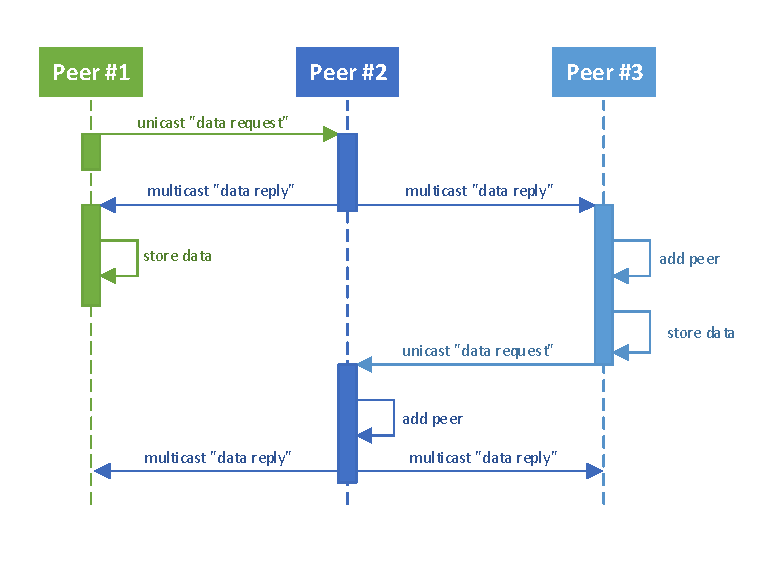
\includegraphics[width=\textwidth]{diagrams/piece-exchange.pdf}
    \caption[Sequence diagram of multicast piece delivery]{Sequence diagram of multicast piece delivery. The multicast \texttt{data reply} allows multiple peers to receive piece data, and also act as implicit local peer discovery announcements.}
    \label{fig:distribution:multicast}
\end{figure}

\section{Conclusion}
\label{sec:distrib:conclusion}
The file is subdivided into fixed-size pieces, which can be distributed over the \gls{P2P} network independently. All information about these pieces is contained in the \gls{torrent-desc}, which must be delivered to every node in some way before starting the torrent download. The SHA-1 hashes of every piece allow a peer to verify the integrity of every piece and, by extension, the entire file.

Peers try to connect with their discovered peer in order to exchange pieces. They maintain some state about what pieces are available at the other end, and which pieces are currently being requested by connected peers. Peers periodically send \texttt{have} messages to keep other peers informed about their download progress, and to indicate that they are still alive.

Pieces are exchanged using a simply request-reply protocol, where one peer sends requests for a part of a piece and the other peer replies with the corresponding data. After all the data of a piece is received, the peer compares the calculated SHA-1 hash with the expected hash from the \gls{torrent-desc}. When the verification succeeds, the peer can request its next missing piece and start serving requests for the received piece itself.

To exploit the locality of peers discovered through local peer discovery, peers send their data replies destined to a local peer to \emph{all} local peers using a link-local multicast. Receiving peers attempt to piggy-back onto this piece exchange, allowing a single piece request to serve many local peers. This enables a faster and more efficient distribution inside clusters of nodes.

\chapter{Prototype implementation}
\label{cha:implementation}
This chapter discusses the prototype implementations of the tracker and the peer which will be evaluated in chapter \ref{cha:evaluation}. These implement the protocol designs from chapters \ref{cha:discovery} and \ref{cha:distribution}, and provide a working example of the protocol in action.

Section \ref{sec:impl:architecture} introduces the system architecture of the prototype. Section \ref{sec:impl:tracker} goes in-depth about the tracker's implementation, followed by the peer implementation in \ref{sec:impl:peer}. Some limitations of the prototype are outlined in \ref{sec:impl:limitations}, ending with a conclusion in section \ref{sec:impl:conclusion}.

\section{System architecture}
\label{sec:impl:architecture}

\subsection{Components}
Figure \ref{fig:impl:architecture} shows the types of components making up the NanoTorrent system. 

The tracker implementation is discussed in section \ref{sec:impl:tracker}. This is responsible for managing the swarms of all torrents, and providing information about these swarms to requesting peers through the NanoTracker protocol. It is assumed to run on a network outside of to the \gls{WSN}.

The peer implementation is detailed in section \ref{sec:impl:peer}. Peers must join the \gls{P2P} network, discover other peers, exchange information about available pieces and exchange missing pieces among each other. They communicate with each other through the NanoTorrent protocol.

A border router is needed to allow communications with the tracker since it is located on an external network. This border router provides the bridge between the \gls{6LoWPAN} communications on the \gls{WSN} and the pure \gls{IPv6} transmissions on the outside network. It also acts as the `root' node for the \gls{RPL} routing protocol used inside the \gls{WSN}. Since it is a common component in many \glspl{WSN} platform, it has a standard implementation in Contiki and is used as-is in the prototype architecture.

\begin{figure}
    \centering
    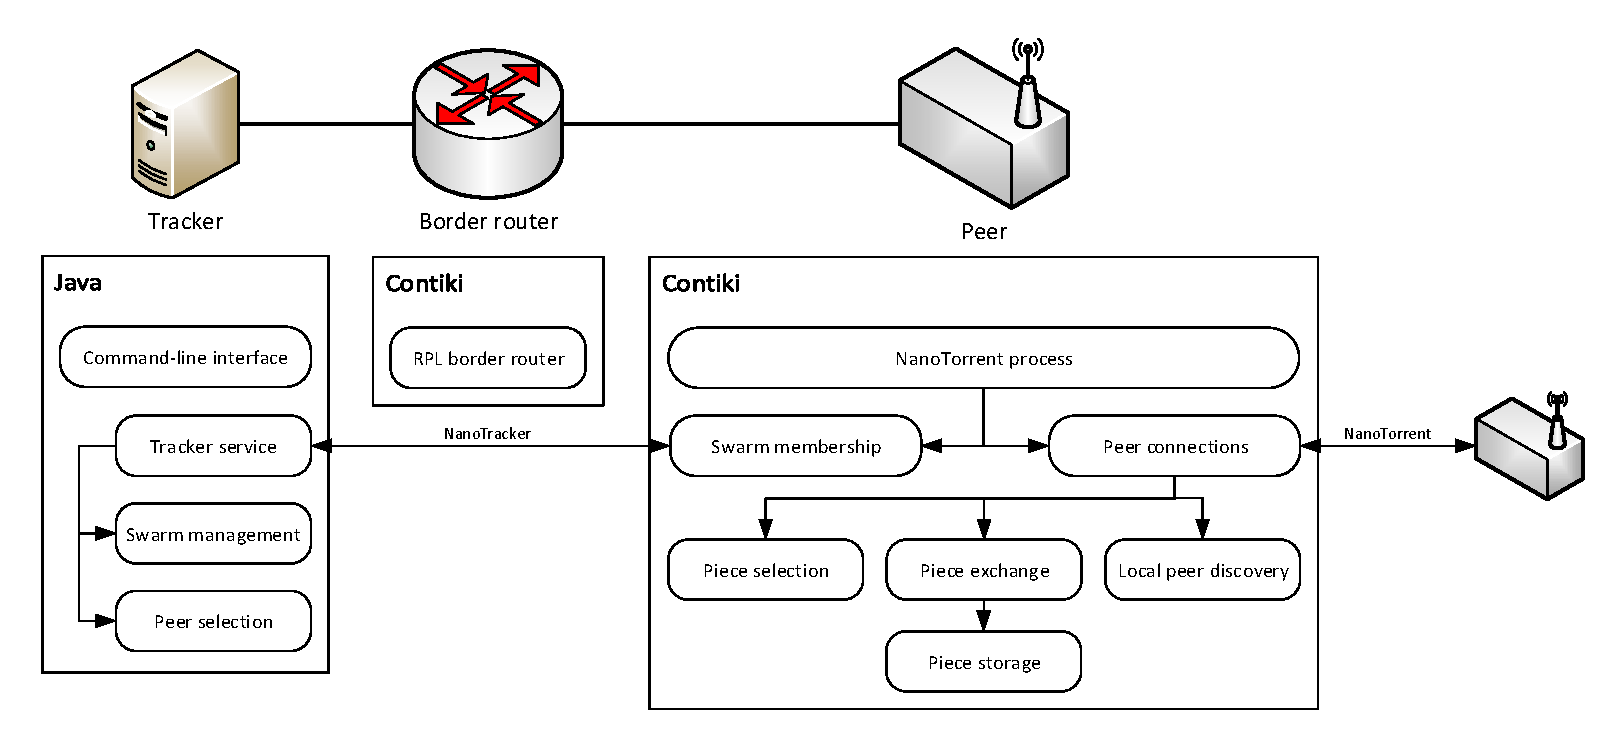
\includegraphics[width=\textwidth]{diagrams/protocol-architecture.pdf}
    \caption{NanoTorrent system architecture}
    \label{fig:impl:architecture}
\end{figure}

\subsection{Communications}
Figure \ref{fig:impl:protocol-overview} gives an overview of all protocol communications between these components in a \gls{WSN} infrastructure.

Peers start off by sending an announce request (1) to the tracker, which must be routed through the border router. The tracker replies with an announce reply (2) containing a list of peers to connect with.

From there, they can initiate peer connections with these discovered peers by sending an initial \texttt{have} message (3). They exchange information about available pieces, and send piece requests for missing pieces (4).

Peers can also discover neighbouring peers through local peer discovery (5), after which they can go through the same process of setting up a peer connection (6) and exchanging pieces (7).

\begin{sidewaysfigure}
    \centering
    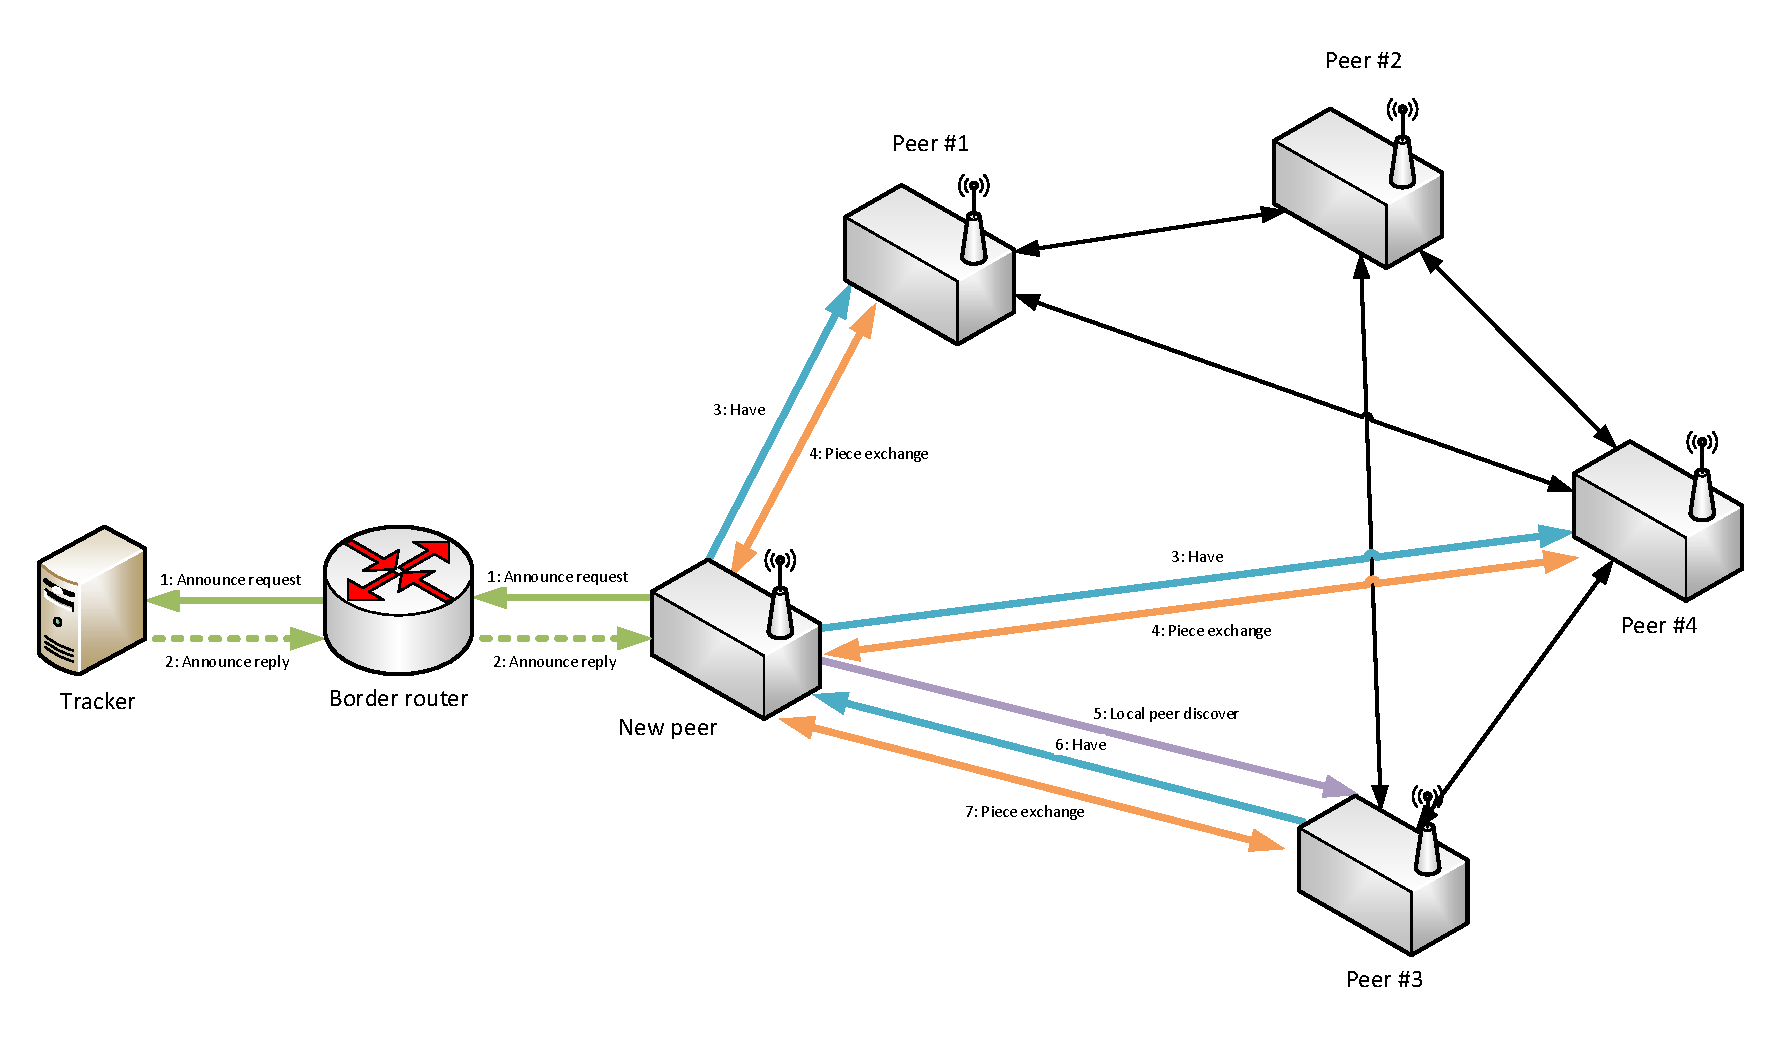
\includegraphics[width=\textwidth]{diagrams/protocol-overview.pdf}
    \caption{Overview of the NanoTorrent protocol communications in a \gls{WSN}}
    \label{fig:impl:protocol-overview}
\end{sidewaysfigure}

\section{Tracker}
\label{sec:impl:tracker}
The tracker described in section \ref{sec:discovery:tracker} is implemented as a standalone Java application. It starts a service to handle incoming NanoTracker announce requests, and provides a basic command-line interface to inspect its \glspl{swarm}.

Its implementation consists of a tracker service component for communications, a swarm manager to retain stateful information, and a peer selection algorithm to generate the peers lists for announce replies.

\subsection{Tracker service}
The tracker service provides the communication endpoint for peers wanting to join or leave a torrent's swarm. It is responsible for parsing incoming announce requests, triggering the needed operations in the managed swarms, collecting the information needed for the announce reply and then sending the reply.

The service listens on a user-specified \gls{UDP} port for incoming announce requests, which must be known by all peers wishing to communicate with this tracker. \gls{UDP} was chosen as underlying transport protocol rather than \gls{TCP}, as NanoTracker is a purely request-reply protocol with no need for long-term conversational state.

\subsection{Swarm management}
The tracker must manage stateful information about the torrent swarms that it is tracking. For every swarm, it retains information about the owning torrent (identified by its \gls{torrent-info-hash}) and the list of peers currently participating in the swarm. For every peer, the tracker records its \gls{IPv6} address, its current membership state and the time of the last received announce request.

When the tracker service receives a request for a torrent with an unknown \gls{torrent-info-hash}, it automatically creates a new swarm for that torrent to start tracking it. This is useful for quickly testing the prototype implementation: the tracker can just be started without any additional set up.

After looking up the swarm corresponding to the request's torrent, the tracker looks up the peer in the swarm based on its \gls{IPv6} address. If the peer is not yet in the swarm, it is added to it. The tracker updates its view on the peer's membership state using the reported state in the announce request, and refreshes the timestamp of its last announce request.

The tracker uses the timestamp of the last announce request sent by each peer to periodically purge non-responsive peers. When a peer fails to send its periodic announce requests to the tracker, its last announce timestamp does not get refreshed. The tracker can detect this and remove these peers. This ensures that peers will only discover peers that have recently refreshed their swarm state, and are likely to still be online when the peer tries to connect with them.

\subsection{Peer selection}
When the announce request is fully processed and the swarm's state is fully updated, the tracker service must reply to the request with a list of peers from the same swarm. This peers list is then used by the receiving peer to connect with other peers in the swarm.

In the current prototype, the tracker doesn't perform any special selection when generating the list of candidate peers. The tracker simply takes a random subset from the swarm, ensuring that this subset is no larger than the requested number of peers and does not include the requesting peer itself. A more intelligent selection algorithm could take advantage of additional information, for example it could prevent a seed from being connected to another seed (as these would have nothing to exchange with each other) or it could maintain a graph representation of the swarm to ensure that every peer is always directly or indirectly connected to a seed.

The generated peers list is used to construct an announce reply, which is then sent back to the peer by the tracker service.

\section{Peer}
\label{sec:impl:peer}
The peer implements the file distribution mechanisms described in chapter \ref{cha:distribution}, the requester's side of the centralized peer discovery from section \ref{sec:discovery:tracker} and the local peer discovery of section \ref{sec:discovery:local}. It is implemented in C on the Contiki platform \cite{contiki}, allowing for cross-compilation to many types of \gls{WSN} platforms.

\subsection{NanoTorrent process}
The main entry point for the peer's implementation is the NanoTorrent main process. This lightweight process initializes all other processes, such as the swarm process maintaining the connection with the tracker and the peer process maintaining connections with other peers. It also reads the list of peers retrieved from the swarm and uses them to initiate new peer connections.

\subsection{Swarm membership}
The swarm membership component is responsible for tracking the peer's membership state, maintaining the connection with the tracker (by periodically sending refreshes) and exposing the retrieved list of discovered peers to the main process.

The client starts a lightweight process to first join the swarm and then send periodic refreshes to the tracker. If it doesn't receive an announce reply after a number of retries, it assumes that the tracker has become unavailable or unreachable and marks itself as having left the swarm.

When the client discovers new peers through the tracker's announce replies, it temporarily stores them in a list while waiting for the main process to try and connect with them. The main process doesn't have to connect with all of the discovered peers, but can let the swarm process hold on to some of them until one of the current peer connections is lost and needs to be quickly replaced.

The main process is notified whenever the membership state changes, e.g. the client has successfully joined the swarm or when the client unexpectedly drops out of the swarm due to connection issues. These inter-process notifications ensure that the main process is aware of the state of all components, and can react when something goes wrong (e.g. losing the connection wit the tracker).

\subsection{Peer connections}
All peer connections and their messages are managed by the peer process. This process maintains a single \gls{UDP} socket listening on a fixed port (same for all NanoTorrent peers), parses the incoming peer messages and handles them for their various purposes: accepting new connections, responding to piece data request and discovering local peers. It is also responsible for the periodic \texttt{have} announcements to all connected peers.

The state that needs to be maintained for every peer connection is described in \ref{sec:distrib:connection}, and the used memory structures maintained by the process directly map onto this description. Peers keep track of the `heartbeat' of every connected peer using individual timers, which are refreshed on every received message. When a heartbeat timer expires, the peer drops the connection.

In order to keep the protocol scalable as the network size increases, peers limit the number of simultaneously opened peer connections. This prevents peers from opening or accepting too many connections, which all need network traffic and thus battery power to be maintained. The client uses two fixed-size `pools' for allocating peer connection states: one for incoming connections and one for outgoing connections. Rather than allocating memory for a new connection dynamically on the heap (e.g. using C's \texttt{malloc}), these pools are allocated in static memory and have a more predictable behaviour.

When a pool is exhausted, newly requested connections cannot be instantiated and these connections must be closed. However, exhaustion of one pool does not affect the other pool. For example, when a client initiates many outgoing connections with peers discovered locally, it can still accept incoming connections from other peers who discovered the client through the tracker.

\subsection{Piece selection}
Whenever a new peer connection is opened or an existing connection is updated with new information about available pieces, the peer process checks if it can request a missing piece on this connection.

Peers use a rarest-first policy for deciding which piece to select next, as described in \ref{sec:distrib:exchange}. To implement this, a client tracks the amount of occurrences of every piece at each of its peers, and finds the piece with the least amount of occurrences (excluding zero occurrences). Whenever a peer connects or disconnects, their available pieces are added or subtracted from the list of piece occurrences.

Peers make sure to not request the same piece from two connections at a time. This is managed in a shared variable, which is modified when new requests are made or old requests are finished. However, when a peer has received almost all of the pieces in a torrent, it is not desirable having to wait on just one peer to deliver the last piece. In this case, the peer goes into what BitTorrent calls \emph{end-game mode}: when nearing completion, a single piece may be requested from more than one connection. The impact of this is minimal as it only occurs at the very end of the download, but makes sure that peers can quickly transition from almost done to fully seeding.

\subsection{Piece exchange}
When a peer discovers an interesting piece at another peer, it can request this piece and start downloading it as detailed in section\ref{sec:distrib:exchange}.

Piece requests are managed individually per connection, with different retry counters and timers for the multiple outstanding requests. This allows parallel requests to operate independently from each other, preventing a single failing connection to take down all connections.

Piece replies destined to local neighbours are sent as multicast packets rather than unicast packets, as specified in \ref{sec:distrib:multicast}. Since the only change is in the destination \gls{IPv6} address, this is readily implemented as a small special case.

\subsection{Piece storage}
The piece data received in piece data replies is written to a file in the \acrfull{CFS}. The client uses the piece index and the piece data offset to calculate the byte offset in the file, and writes the bytes from the reply into the file. Similarly, data is read from the file when sending a piece data reply.

On the AVR Zigduino platform, \gls{CFS} is configured to use the \gls{EEPROM} for file system storage. This allows for 4 KB of read/write storage \cite{zigduino-manual}, which is sufficient for most network reprogramming or reconfiguration use cases. For experiments in the COOJA simulator \cite{cooja}, \gls{CFS} uses an in-memory file system.

\subsection{Local peer discovery}
Peer discovery through local multicast as discussed in section \ref{sec:discovery:local} is implemented as a modification to the periodic \texttt{have} announcements. Rather than sending the \texttt{have} announcements to individual local peers, it is multicasted to all local neighbours.

Incoming \texttt{have} multicast announcements are handled as regular incoming connection requests. The peer will try to accept the connection (if it hasn't already), and will process the message if it has a connection. As noted in \ref{sec:distrib:connection}, peers must not reply with a \texttt{close} message if it fails to accept a connection in response to a multicast \texttt{have}. Other than that, it can treat local peers and remote peers uniformly.

\section{Usage}
\label{sec:impl:usage}

\subsection{Deployment}
In order to deploy NanoTorrent onto a \gls{WSN}, the network operator must deploy the tracker on a computer on an external network, deploy a Contiki application using NanoTorrent onto the \gls{WSN} nodes and connect the external network with the \gls{WSN} with a border router.

\subsubsection{Tracker}
The tracker is a simple Java command-line application which can be started to operate on any \gls{UDP} port. The computer on which it is deployed must have a Java runtime installed and must have a connection with the border router. Other than that, the tracker is very much `fire and forget': it can run in the background and doesn't need user interaction.

\subsubsection{Peer}
The prototype is implemented in C for the Contiki platform, so it must be compiled for the particular platform used by the \gls{WSN} nodes. The implementation does not rely on hardware-specific features, so it can readily be cross-compiled to any of Contiki's supported platforms -- although it is recommended to fine-tune the protocol's configuration to the specifics of the used platform.

The prototype comes with a demo application, which has been verified to run on both the AVR Zigduino platform and in the COOJA simulator environment. The demo is implemented in \texttt{peer/demo.c} and can be compiled with the Makefile rule \texttt{demo}.

\subsubsection{Border router}
The \gls{RPL} border router is a standard component in Contiki, and can be found in \texttt{contiki/examples/ipv6/rpl-border-router}.

\subsection{Bootstrapping}
Before peers can start downloading a torrent, they must have received the \gls{torrent-desc} from the distributor, as explained in \ref{sec:discovery:torrent-desc}. The torrent descriptor is needed to `bootstrap' the NanoTorrent client, as it contains vital information needed for the file distribution. In the case of BitTorrent, the distributor creates and publishes a \texttt{.torrent} file containing the torrent's metainfo, as mentioned in section \ref{sec:related:bittorrent}. Users download this \texttt{.torrent} file and open it with a BitTorrent client to start the download.

\subsubsection{NanoGen toolchain}
The distributor can use the included NanoGen tool to generate a torrent descriptor file to be distributed to all destined NanoTorrent nodes. NanoGen takes as input the file to be distributed, details about the tracker and the piece size and produces a binary file which can be parsed by the NanoTorrent prototype implementation. The tool takes care of subdividing the input file into pieces of the given size, calculating the SHA-1 hashes of every piece and writing them to the output file.

To inspect the contents of a generated torrent descriptor file, the NanoRead utility was added. This utility takes a torrent descriptor file as input and prints its contents in a human-readable format. This is useful for verifying the contents of a generated or download torrent descriptor, and for debugging purposes.

NanoGen and NanoRead are implemented in C as Contiki applications in \texttt{peer/nanogen.c} and \texttt{peer/nanoread.c}. They can be compiled through the Makefile rules \texttt{nanogen} and \texttt{nanoread} with the flag \texttt{TARGET=native} to compile for the native platform (e.g. Linux). These rules produce executables for the command-line applications named \texttt{nanogen.native} and \texttt{nanoread.native}.

\subsubsection{Torrent descriptor distribution}
The current prototype implementation does not provide a mechanism for distributing a torrent descriptor. Like BitTorrent, the NanoTorrent client requires that the descriptor is available locally on the node, and is not concerned with \emph{how} the descriptor is retrieved.

For evaluation and demonstration purposes, the torrent descriptor is hard-coded into the NanoTorrent image at compilation time. The Makefile rule for the demo application takes a \texttt{TORRENT\_DESC} argument which specifies the path to the torrent descriptor file. This file is written in the static file system section of the created demo image, which will be read by the demo application at node start up.

\subsubsection{Seed configuration}
In order to configure a node act as a seed, it must have the whole file available at start up. NanoTorrent clients use the \acrfull{CFS} for storing the distributed file, so the seed must have the file prepared in its local file system.

On the AVR Zigduino platform, \acrfull{CFS} is configured to use the \gls{EEPROM} for file system storage. The Makefile provides the \texttt{demo.seed} rule to generate an \gls{EEPROM} image for the file system with the given \texttt{TORRENT\_FILE} at the start of the \gls{CFS} region. A seed can then be flashed with the \texttt{demo.seed.eu} and \texttt{demo.seed.u} rules.

For evaluating the NanoTorrent implementation in the COOJA simulator \cite{cooja}, the distributed file must be uploaded to the appropriate NanoTorrent nodes through COOJA's mote configuration interfaces.

\section{Limitations}
\label{sec:impl:limitations}
The current implementation is very much just a prototype. Many features common in mature file distributions are missing or are not fully fleshed out.

\subsection{Bootstrapping}
Currently, the torrent descriptor is hard-coded into the peer's program during compilation, locking the peer into downloading just one file. A more complete network reprogramming solution based on NanoTorrent should include a more versatile distribution mechanism for this descriptor.

The particularities of such mechanism depend heavily on the used \gls{WSN} middleware platform. For example, a \gls{WSN} running on the LooCI \cite{looci} platform would communicate mostly through LooCI's event-based communication network. A reconfiguration engine based on NanoTorrent for LooCI could send the torrent descriptor as payload data of a LooCI event, and have them launch the NanoTorrent process in response.

\subsection{Security}
The prototype assumes that nodes in the network can be trusted. Although this assumption is defendable in the context of experimental \glspl{WSN}, it does not hold for large-scale deployments where malicious peers could attack the network from the outside or the inside.

For example, a malicious node could intentionally send corrupted piece data to a peer, causing it to write the wrong data to its file. The peer will detect the corruption only after it has fully received the piece (possibly through multiple data requests), and will need to request the same piece again.

The tracker is also susceptible to uncontrolled announce requests. Every time a new request arrives for an unknown torrent, the tracker creates a new swarm and starts tracking it. This is sufficient for small-scale experimental uses, but could be abused by sending many announce requests with bogus torrent info hashes. The tracker would allocate a lot of swarms which are never used and never cleaned up, potentially crashing it due to it running out of memory. To prevent such abuse, trackers deployed in the wild should only accept announce requests for known torrents registered in a backing database.

\section{Conclusion}
\label{sec:impl:conclusion}
The prototype for the tracker and the peer provides the basic implementation of the protocol designs from chapters \ref{cha:discovery} and \ref{cha:distribution}, taking into account the constraints and limitations imposed by \gls{WSN} nodes. It comes with tools for generating and inspecting torrent descriptors, monitoring the swarms on the tracker and compiling images for NanoTorrent leechers and seeds.

The prototype lacks additional features commonly found in more mature file distribution mechanisms, such as an easy-to-use bootstrapping process or security checks. However, it provides enough to do useful evaluations of the proposed protocol in small experiments.

\chapter{Evaluation}
\label{cha:evaluation}
This chapter evaluates the prototype implementation of the NanoTorrent protocol.

Section \ref{sec:eval:hypotheses} lists the formed hypotheses that need to be evaluated. Section \ref{sec:eval:method} describes the evaluation methodology. Section \ref{sec:eval:scale} evaluates the scalability of the protocol, and section \ref{sec:eval:hetero} tests the protocol in a heterogeneous deployment. Section \ref{sec:eval:improvements} lists possible improvements that could be made to the protocol, and \ref{sec:eval:discussion} concludes with a discussion.

\section{Hypotheses}
\label{sec:eval:hypotheses}
The goal of NanoTorrent is to deliver files to many \gls{WSN} nodes in a reasonable amount of time, while remaining efficient on battery usage. It should be able to achieve this for many network topologies, which may possibly consist of different types of nodes -- not all of them running a NanoTorrent implementation.

To allow for both fast distribution and heterogeneity in the network, NanoTorrent approaches this problem with a \gls{P2P} file distribution protocol supported by a hybrid peer discovery mechanism. The use of both local peers and remote peers should allow for fast distribution among neighbouring nodes, while still enabling piece exchange with faraway nodes which can help spreading the file in other parts of the network.

\section{Methodology}
\label{sec:eval:method}
To test these hypotheses, the NanoTorrent implementation is run in various experiment configurations inside the COOJA simulator. In each experiment, nodes are tasked to distribute a given torrent and must fully retrieve and verify the contents of the distributed file.

\subsection{AVR Zigduino}
The prototype has been tested and verified in a small network with AVR Zigduino nodes consisting of one border router, one initial seed and three regular peers. The border router is connected to a laptop running the tracker implementation.

Although this set up works, it does not allow a very thorough evaluation of the protocol's capabilities to scale up to larger networks.

\subsection{COOJA simulator}
The evaluations were performed in the COOJA simulator \cite{cooja}. This is a simulation environment for Contiki nodes that emulates the hardware layer of a Contiki platform. It allows Contiki applications to be cross-compiled with the COOJA-specific hardware implementation, and can run these specially compiled versions in various simulated conditions.

COOJA comes with the Contiki distribution and is implemented as a Java application. The simulator interface allows the user to add new motes, place them in a simulated wireless network and configure them. While running a simulation, COOJA shows and records the message logs of all nodes, the timeline of occurred events and the packets transmitted across the network. The recorded information can also be exported for in-depth analysis by other tools.

COOJA simulates the platform and the network at the hardware layer, and interfaces with the compiled C code through the \gls{JNI}. This allows COOJA to run almost any Contiki application, as it behaves just like any other target Contiki platform for cross-compilation. This method of full system simulation is more faithful to real platforms than other simulators such as TOSSIM \cite{tossim} which can only simulate one layer of the platform.

\section{Scalability}
\label{sec:eval:scale}
To be usable in both small-scale experimental setups and large-scale \gls{WSN} deployments, NanoTorrent must be able to scale as more nodes are added to the network.

\subsection{Set up}
Figure \ref{fig:eval:scale:setup} shows the simulation set up. In each experiment, $N^2$ nodes are deployed in an $N \times N$ grid layout such that each node has at most 4 neighbours. Every node has a torrent descriptor for a 2 \gls{KB} file consisting of 8 pieces of 256 \gls{KB}. The top left node acts as the \gls{initial-seed} from which this file will start propagating over the network. This node is also connected with a border router, which connects the \gls{WSN} with the \gls{tracker}. The experiment was carried out for $N =$ 3 to 7, resulting in networks consisting of $9$ to $49$ NanoTorrent peers.

Since all nodes in this set up download the same torrent, file distribution could also be done \emph{without} a centralized tracker. To analyse the benefits or downsides to this approach, every set up is tested once without the tracker and once with both peer discovery mechanisms enabled.

\begin{figure}
    \centering
    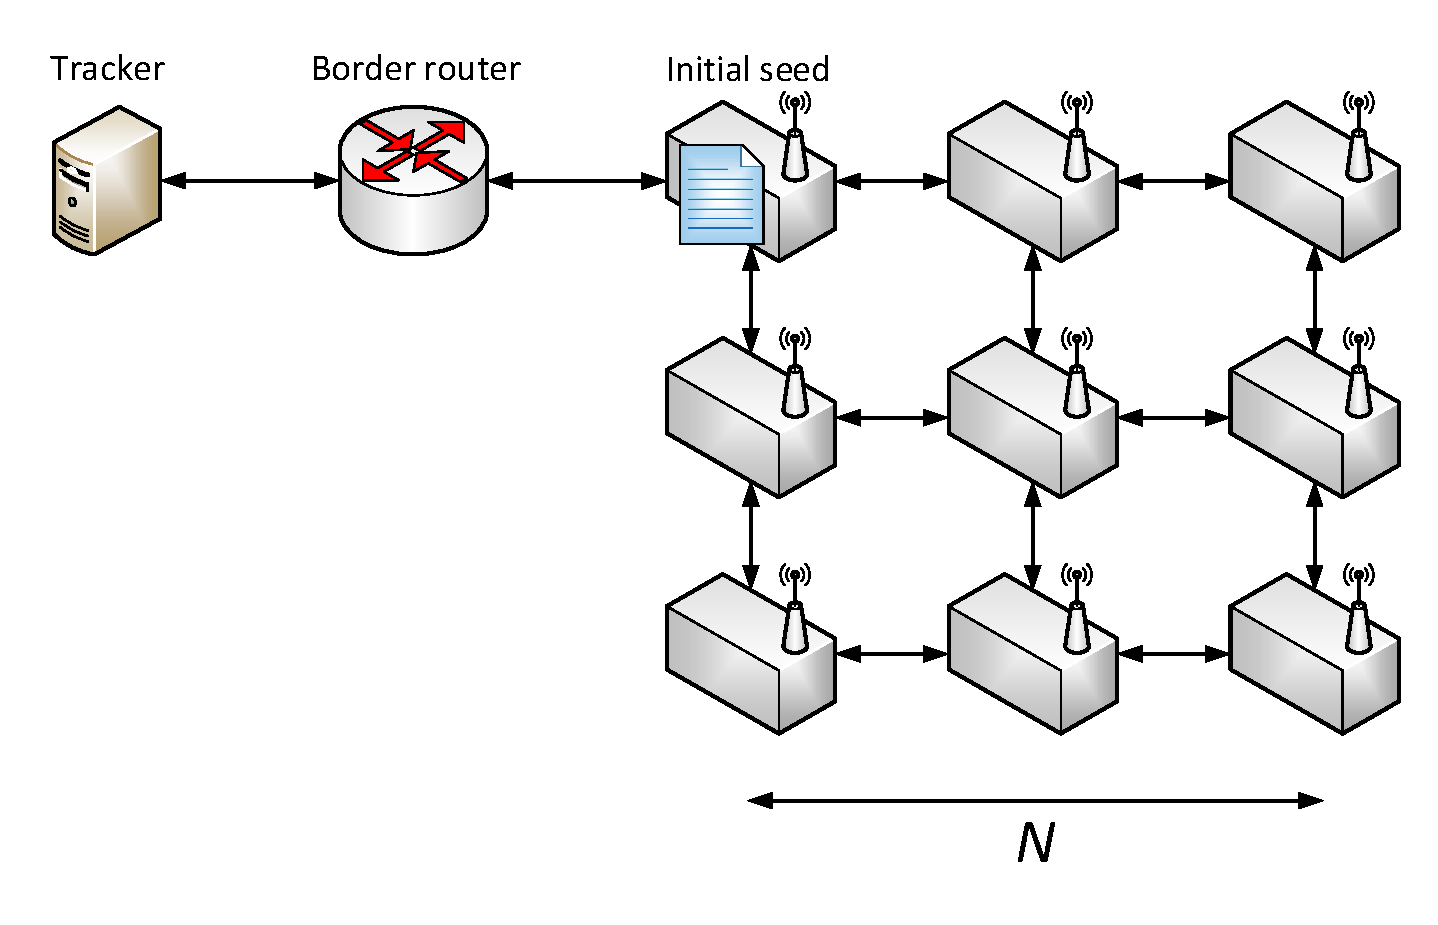
\includegraphics[width=\textwidth]{diagrams/experiment-scale.pdf}
    \caption[Network set up for scalability experiment]{Network set up for scalability experiment. The \gls{WSN} consists of $N \times N$ nodes in a grid layout, with one initial seed.}
    \label{fig:eval:scale:setup}
\end{figure}

\subsection{Results}
Figure \ref{fig:eval:scale:deploy-time} shows the deployment times (i.e. the time to deploy the file to all nodes) for the different network diameters, both with and without the tracker.

Figure \ref{fig:eval:scale:total-transmissions} shows the total number of transmissions sent over the network. This total is broken down into the different upper-layer network protocols in figure \ref{fig:eval:scale:transmissions}. NanoTorrent and NanoTracker indicate messages between peers and with the tracker. \gls{IEEE} 802.15.4 messages consist of link-layer acknowledgements for transmitted frames. \gls{ICMPv6} messages are used to maintain the \gls{IPv6} and \gls{RPL} routing mechanisms. \gls{6LoWPAN} messages consist of fragmented packets which are later re-assembled into larger \gls{IPv6} packets.

Figure \ref{fig:eval:scale:3x3} gives a more in-depth analysis of the download progression in a $3 \times 3$ network. 8 nodes (numbered 3 to 10) receive the file from a single initial seed.

Figure \ref{fig:eval:scale:7x7} displays the completion times of peers in a $7 \times 7$ network. Rather than showing the individual progress of each of the 49 nodes similar to figure \ref{fig:eval:scale:3x3}, this figure only shows the time at which they receive their last missing piece, grouping the results in 5 second intervals. The initial seed is also shown as the only peer completing the torrent after 0 seconds.

\begin{figure}
    \centering
    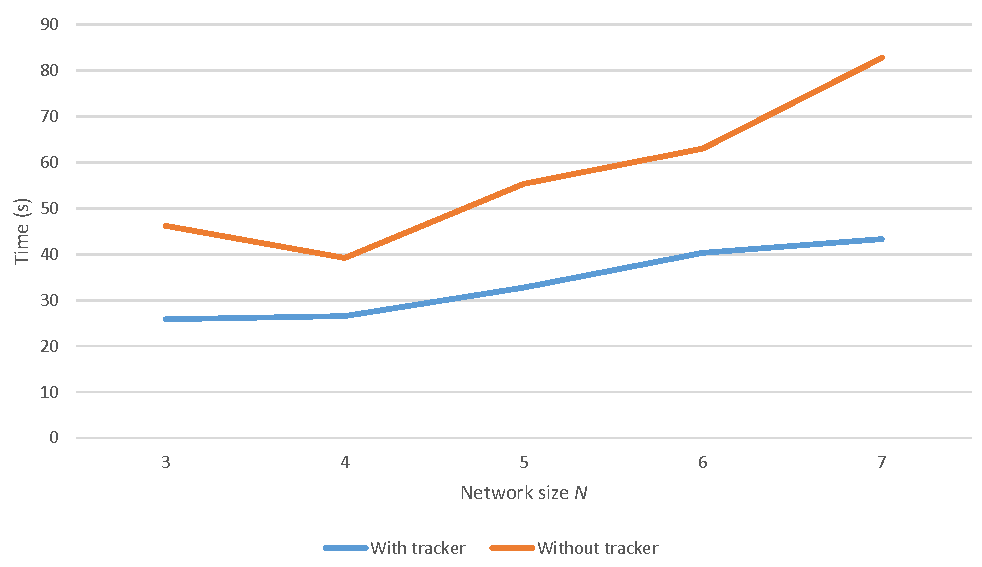
\includegraphics[width=\textwidth]{graphs/scale/deploy-time.pdf}
    \caption[Deployment times for increasing network diameter]{Time to deploy the full file to all nodes for network diameter $N$.}
    \label{fig:eval:scale:deploy-time}
\end{figure}

\begin{figure}
    \centering
    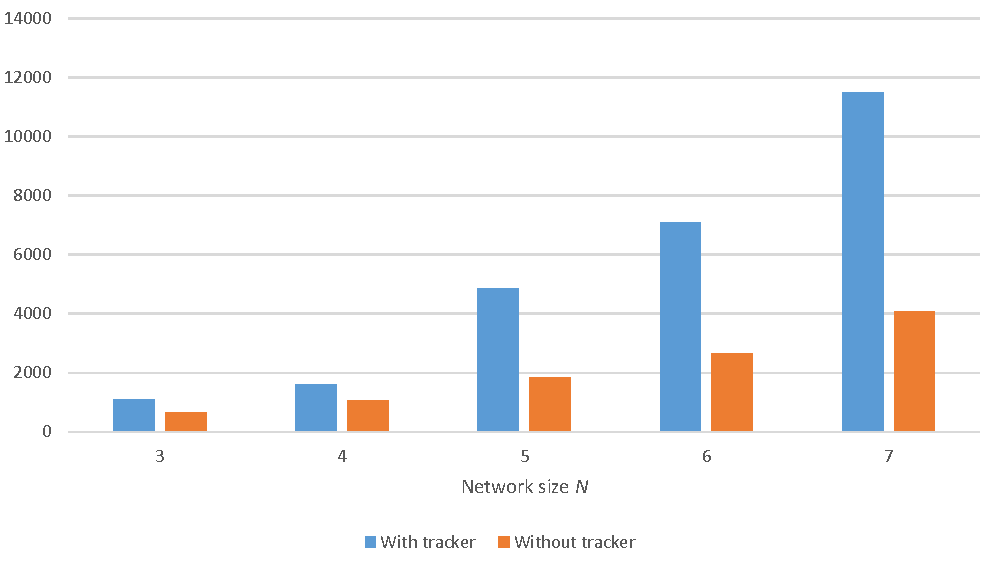
\includegraphics[width=\textwidth]{graphs/scale/total-transmissions.pdf}
    \caption[Total transmissions for increasing network diameter]{Total transmissions sent during deployment for increasing network diameter $N$.}
    \label{fig:eval:scale:total-transmissions}
\end{figure}

\begin{figure}
	\centering
	\begin{subfigure}[b]{\textwidth}
		\centering
		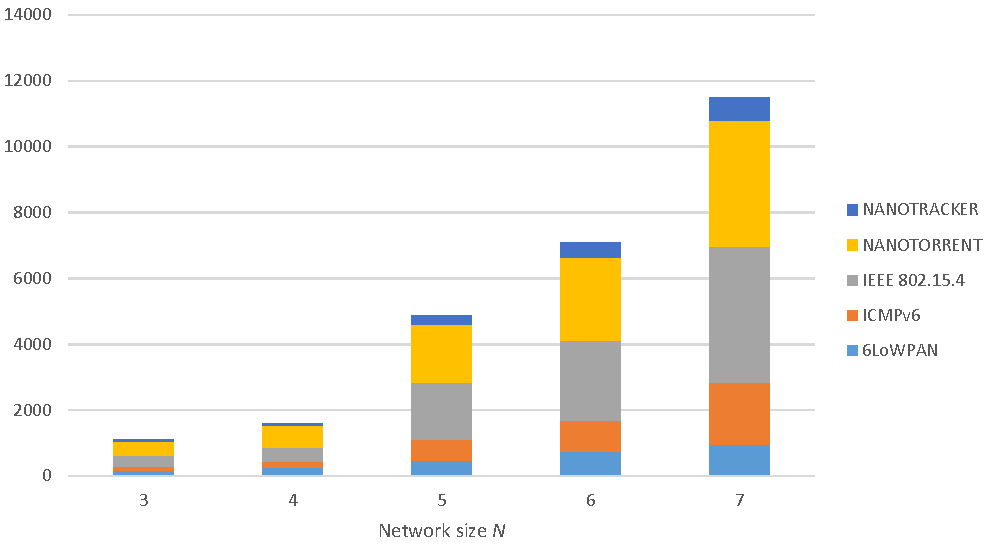
\includegraphics[width=\linewidth]{graphs/scale/transmissions-tracker.pdf}
		\caption{With tracker.}
		\label{fig:eval:scale:transmissions:tracker}
	\end{subfigure}%
	\\
	\begin{subfigure}[b]{\textwidth}
		\centering
		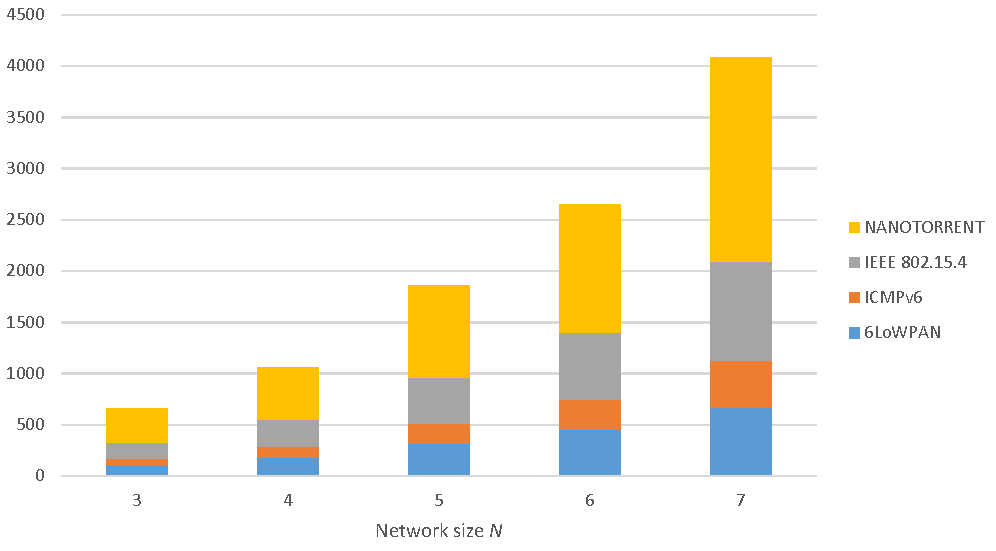
\includegraphics[width=\linewidth]{graphs/scale/transmissions-no-tracker.pdf}
		\caption{Without tracker.}
		\label{fig:eval:scale:transmissions:no-tracker}
	\end{subfigure}
	\caption{Protocol breakdown of transmissions in $N \times N$ network}
	\label{fig:eval:scale:transmissions}
\end{figure}

\begin{figure}
	\centering
	\begin{subfigure}[b]{\textwidth}
		\centering
		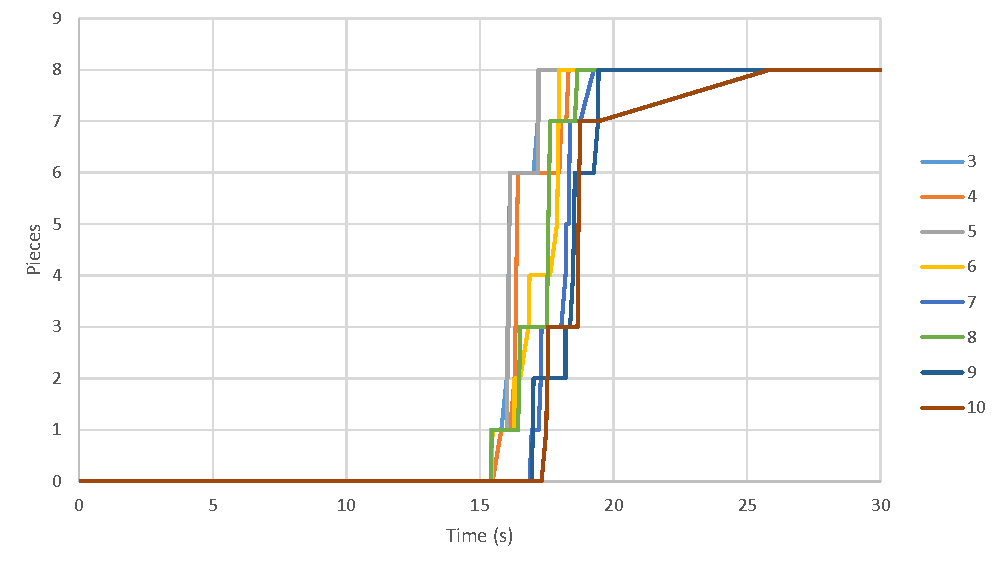
\includegraphics[width=\linewidth]{graphs/scale/tracker-3x3-progress.pdf}
		\caption{With tracker.}
		\label{fig:eval:scale:3x3:tracker}
	\end{subfigure}%
	\\
	\begin{subfigure}[b]{\textwidth}
		\centering
		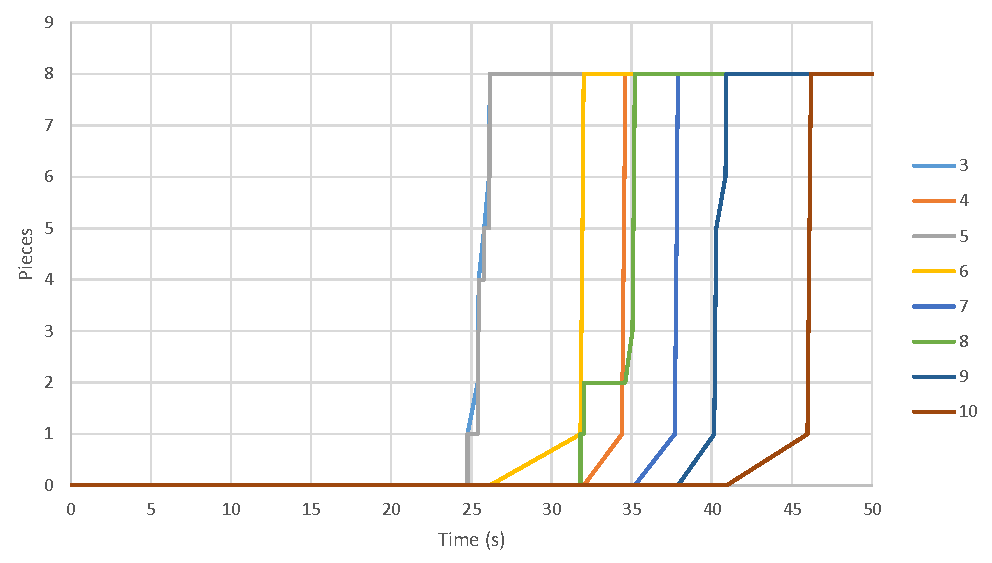
\includegraphics[width=\linewidth]{graphs/scale/no-tracker-3x3-progress.pdf}
		\caption{Without tracker.}
		\label{fig:eval:scale:3x3:no-tracker}
	\end{subfigure}
	\caption[Download progression in $3 \times 3$ network]{Download progression for 8-piece file in $3 \times 3$ network. The different coloured lines indicate the progress of different peers.}
	\label{fig:eval:scale:3x3}
\end{figure}

\begin{figure}
	\centering
	\begin{subfigure}[b]{\textwidth}
		\centering
		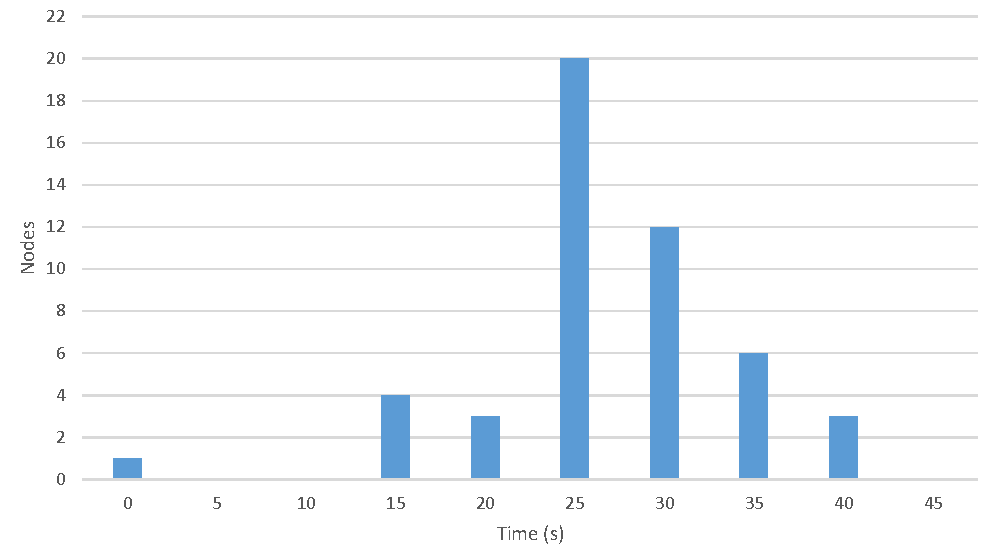
\includegraphics[width=\linewidth]{graphs/scale/tracker-7x7-completion.pdf}
		\caption{With tracker.}
		\label{fig:eval:scale:7x7:tracker}
	\end{subfigure}%
	\\
	\begin{subfigure}[b]{\textwidth}
		\centering
		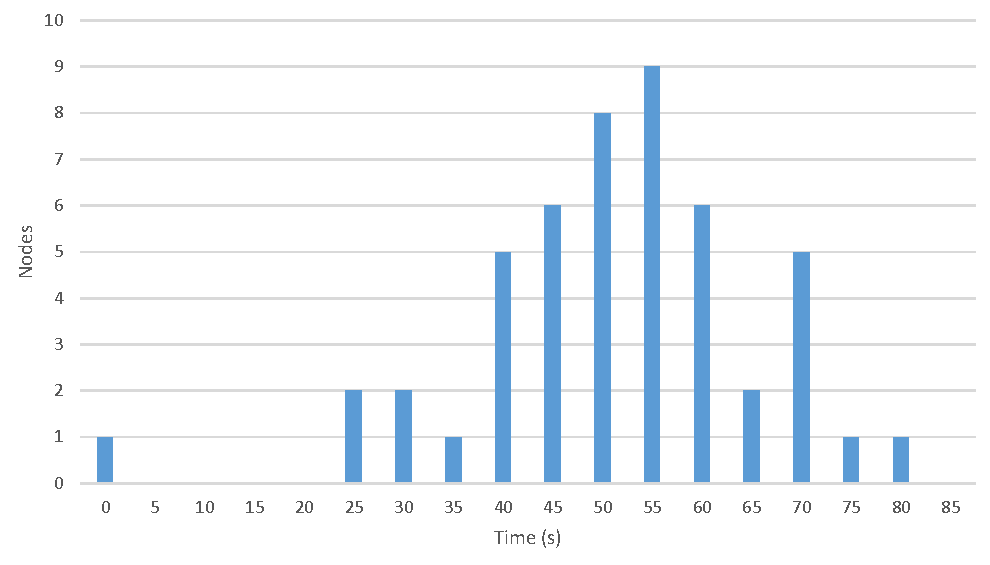
\includegraphics[width=\linewidth]{graphs/scale/no-tracker-7x7-completion.pdf}
		\caption{Without tracker.}
		\label{fig:eval:scale:7x7:no-tracker}
	\end{subfigure}
	\caption[Completion times in $7 \times 7$ network]{Completion times in $7 \times 7$ network. The labels on the X-axis denote the start of an interval, e.g. $0s$ to $5s$.}
	\label{fig:eval:scale:7x7}
\end{figure}

\subsection{Interpretation}
\subsubsection{Deployment time}
Figure \ref{fig:eval:scale:deploy-time} shows that the use of a tracker clearly decreases the total time needed to deploy the file to the whole network. Every peer has additional connections with remote peers from which they can request pieces. Peers on the edge of the network can connect with peers closer to the initial seed, acquire pieces faster and help distribute them to their neighbours.

Without a tracker, every peer must wait until one of its neighbours starts receiving the file. Pieces propagate from the initial seed to the rest of the network as a `wave'. This means that peers on the far edge of the network barely participate in the file distribution, only receiving the file when all other peers have already received it.

Both approaches appear to scale linearly with network size in terms of deployment time. As the network increases in size, the path length between the initial seed and the furthest peer increases linearly as well which is the primary contributor to the deployment time.

\subsubsection{Transmissions}
However, the increased deployment speed from using a tracker comes at a cost in terms of transmitted messages as shown by figure \ref{fig:eval:scale:total-transmissions}. As peers connect with more peers, they need to send more periodic announcements and reply to requests from more peers. While peers on the edge of the network can help balance the load from distributing pieces, communicating with faraway peers is more costly to the network as a whole. The messages between a node and the tracker or its remote peers must traverse the network, taking multiple hops along intermediate nodes which need to use their transmission power to route the \gls{IPv6} packets. These long distance messages account for a lot of overhead transmissions when compared to the tracker-less approach, and this overhead increases with network diameter.

When breaking down these transmissions by protocol, most messages show up as either NanoTorrent or link-layer acknowledgements. The link-layer acknowledgements are an integral part of the network stack, and their usage increases as messages take more hops to get to their destination. This increase is more prevalent in the experiments with a tracker, as NanoTorrent messages need to routed by more nodes to reach a remote peer.

While the number of transmissions without a tracker scales fairly linearly with increasing network size, the number of transmissions when using a tracker seems to increase more than linearly. The additional connections opened by peers cause extra messages on the network which need to be routed across multiple hops.

\subsubsection{Progression}
In the $3 \times 3$ network of figure \ref{fig:eval:scale:3x3:tracker}, all nodes quickly start receiving the file as soon as they receive the first periodic \texttt{have} announcement from the initial seed. Thanks to the tracker, multiple nodes are connected to this initial seed, which means more peers benefit from this initial announcement. In figure \ref{fig:eval:scale:3x3:no-tracker}, the absence of a tracker results in only the two direct neighbours of the seed (nodes 3 and 5) receiving this first announcement. The initial seed communicates only with these two neighbours, which in quick succession request all pieces of the file. However, they take a couple of seconds before notifying their own neighbours, and have already completely downloaded the file before their next \texttt{have} announcement is due. This leaves some room for improvement for fine-tuning the timings of these announcements, to let neighbours more quickly know when new pieces are available.

Figure \ref{fig:eval:scale:7x7} shows the distribution of the completion times of all nodes in a $7 \times 7$ network. For this scenario, the use of a tracker results in a nearly two-fold speed up, distributing the last piece after just 43 seconds as opposed to 82 seconds in the tracker-less experiment. Most peers complete the download around the halfway point, when the `wave front' of the file distribution is the widest at the main diagonal of the grid. In theory, this is when the $N-1$ nodes on the sub diagonal of the square grid are sending pieces to $N$ nodes on the main diagonal, reaching the maximum number of concurrent transfers. When a tracker is employed, the distribution is more skewed as peers use remote connections to exchange pieces.

\section{Heterogeneity}
\label{sec:eval:hetero}
Whereas other distribution protocols for \glspl{WSN} such as Deluge (see \ref{sec:related:deluge}) require all nodes to run the same distribution protocol, NanoTorrent can operate in a \emph{heterogeneous} network consisting of nodes with different tasks and different programs. As long as all nodes properly route \gls{IPv6} traffic across the \gls{WSN}, NanoTorrent peers can communicate with each other even if they are separated by non-NanoTorrent nodes.

\subsection{Set up}
To validate this mode of operation, an experiment was carried out with two clusters each consisting of $5 \times 5$ NanoTorrent peers, which are only connected by a single border router node. This border router routes \gls{IPv6} traffic between the two clusters and to the tracker on the external network. Peers in different clusters can only reach each other through this border router. The set up is shown in figure \ref{fig:eval:hetero:setup}.

\begin{figure}
    \centering
    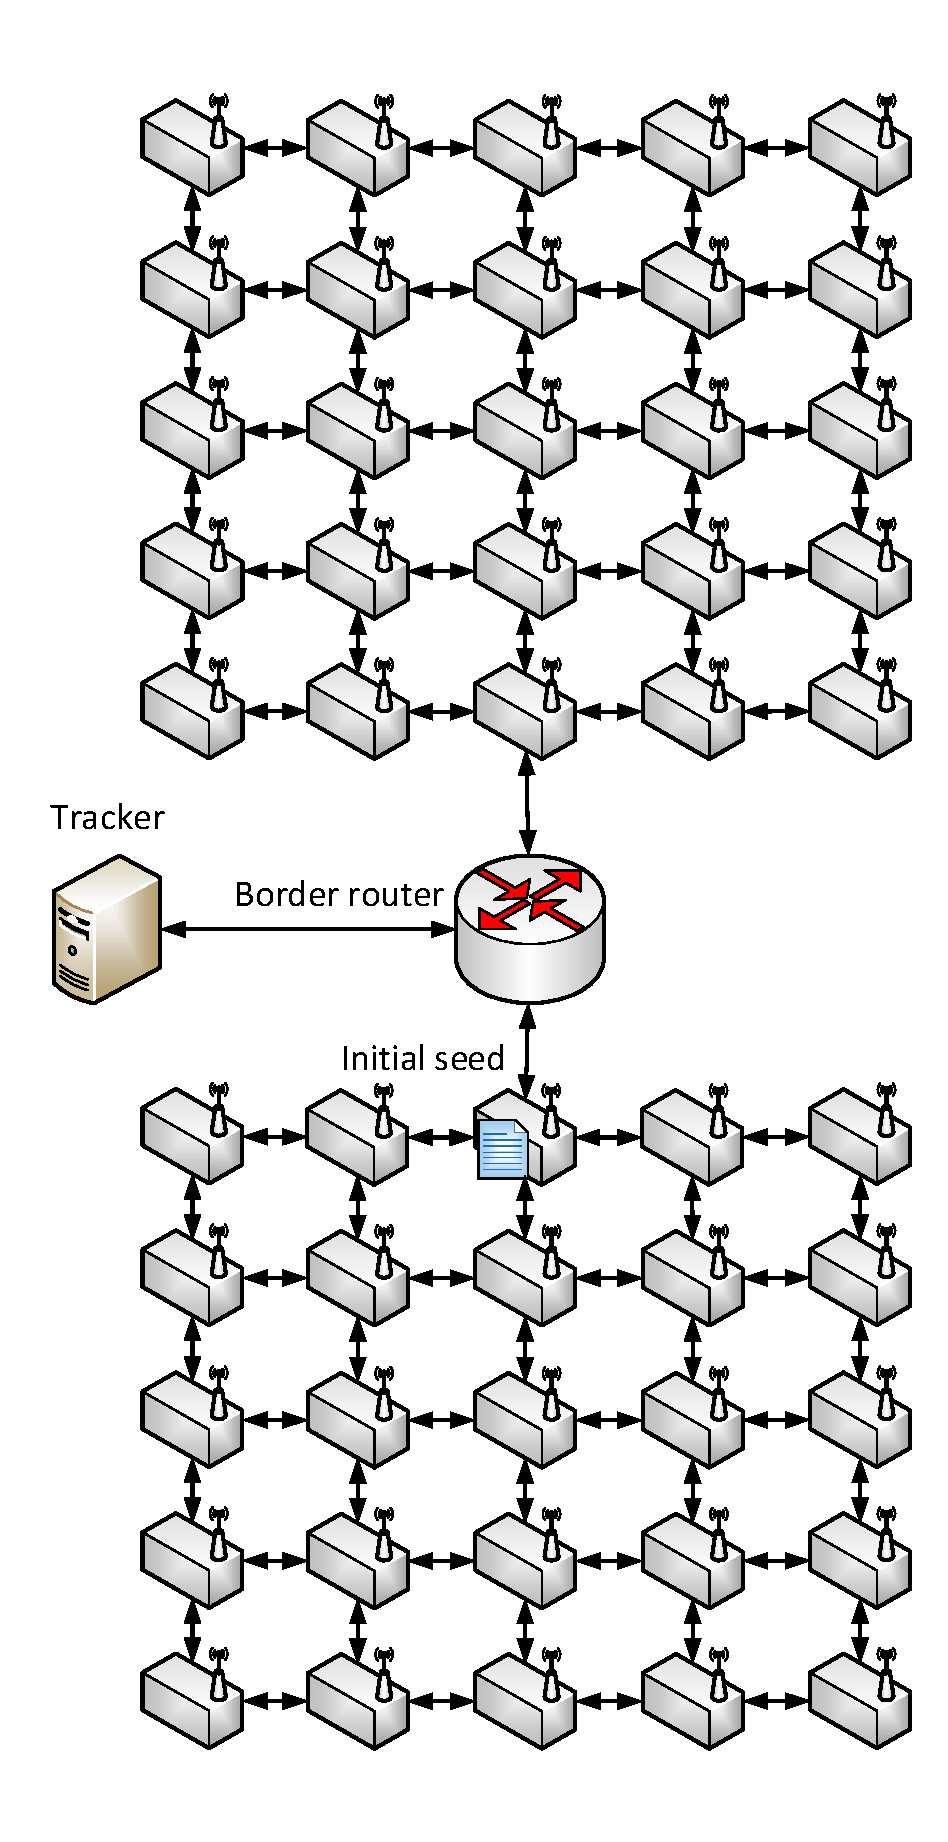
\includegraphics[height=.9\textheight]{diagrams/experiment-cluster.pdf}
    \caption[Network set up for Heterogeneity experiment]{Network set up for Heterogeneity experiment. The \gls{WSN} consists of 2 separate clusters of $5 \times 5$ nodes in a grid layout, with one initial seed in one of the clusters.}
    \label{fig:eval:hetero:setup}
\end{figure}

\subsection{Results}
Figure \ref{fig:eval:hetero:progress} show the download progress of 5 nodes from each cluster of NanoTorrent nodes. Nodes numbered 2 to 26 are in the cluster with the initial seed, while nodes 27 to 51 are in the other cluster.

Figure \ref{fig:eval:hetero:completion} displays the completion times of all the peers in the network, i.e. the time at which a peer receives their last missing piece, grouping the results in 5 second intervals. The initial seed is shown as the only peer completing the torrent after 0 seconds.

\begin{figure}
	\centering
	\begin{subfigure}[b]{\textwidth}
		\centering
		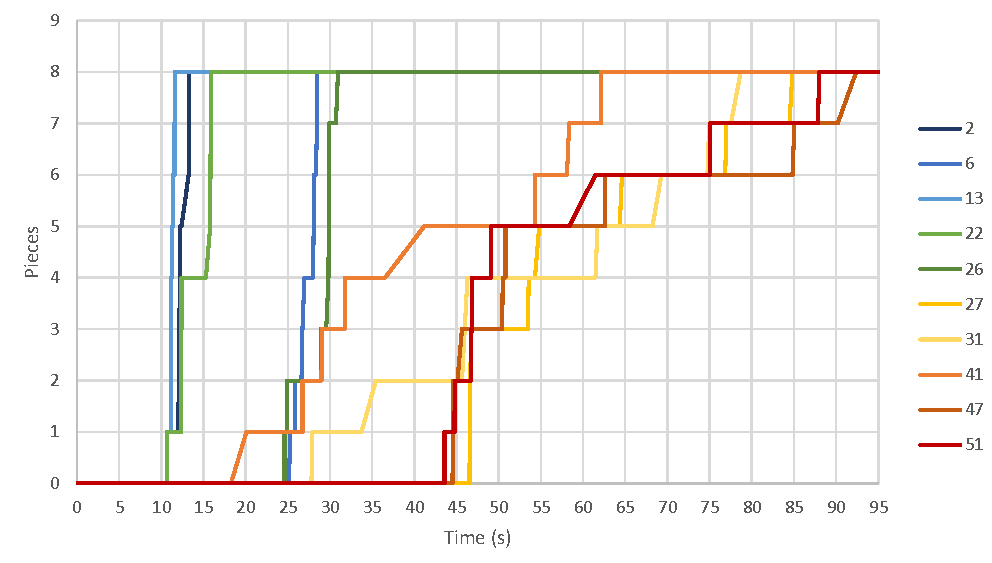
\includegraphics[width=\linewidth]{graphs/cluster/two-cluster-seed-12-progress.pdf}
		\caption{Download progression of a selected number of nodes.}
		\label{fig:eval:hetero:progress}
	\end{subfigure}%
	\\
	\begin{subfigure}[b]{\textwidth}
		\centering
		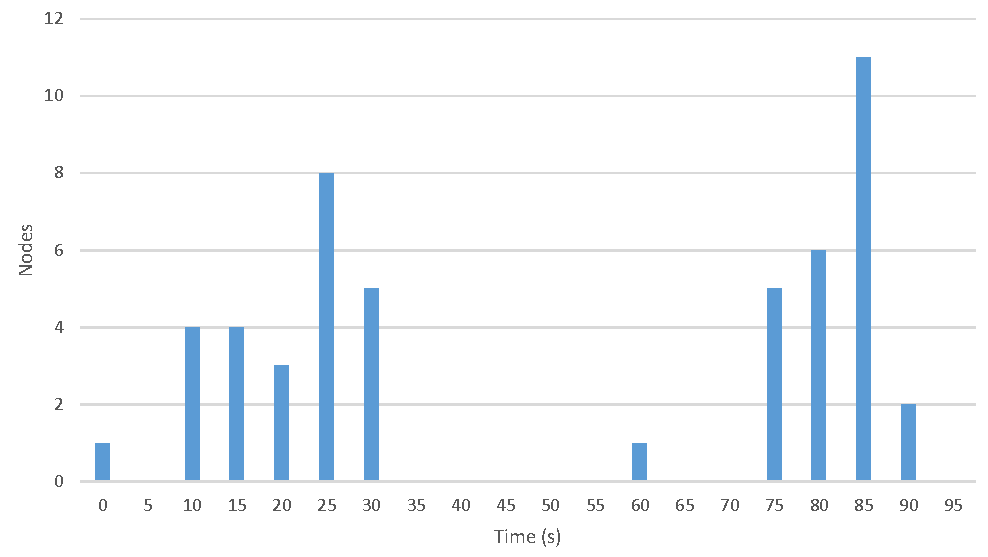
\includegraphics[width=\linewidth]{graphs/cluster/two-cluster-seed-12-completion.pdf}
		\caption{Completion times.}
		\label{fig:eval:hetero:completion}
	\end{subfigure}
	\caption[Results for network consisting of two separate clusters]{Results for a network consisting of two $5 \times 5$ clusters.}
	\label{fig:eval:hetero:results}
\end{figure}

\subsection{Interpretation}
As expected from the results in section \ref{sec:eval:scale}, figure \ref{fig:eval:hetero:progress} shows that peers in the cluster with the initial seed start exchanging pieces quickly. After 35 seconds, the whole cluster has received all pieces of the file and start seeding the torrent.

In the meantime, some nodes in the other cluster manage to connect a peer in the seeding cluster through the tracker and slowly start receiving pieces. Their initial progress is slowed down by the need to pass through the single border router, but quickly start spreading the received pieces to other peers in their cluster. It takes a minute for the first node in this cluster to complete its download, and 30 seconds later the last node receives its last piece.

This slow progression in the second cluster is evident in the distribution of completion times in figure \ref{fig:eval:hetero:completion}. The last node in the seeding cluster completes its download a full 30 seconds before the first node in the other cluster does. Although these nodes do progress, they are fully dependent on the seeding cluster and they are limited by the network.

\section{Possible improvements}
\label{sec:eval:improvements}
There is definitely room improvement for the NanoTorrent protocol. Configuration parameters still need to be tuned, multiple peer discovery mechanisms may discover the same peer multiple times, and piece data transmissions can still be made more efficient.

\subsection{Parameter tuning}
The protocol uses many timers to coordinate its behaviour, most of which still need to be fine-tuned. For example, file distribution only takes off after all nodes are properly initialized and the initial seed sends its first periodic \texttt{have} announcement -- currently after 15 seconds. These 15 seconds at the start of the distribution is time wasted doing nothing useful, delaying the network reprogramming and the return to normal network operation. Increasing the frequency of \texttt{have} announcements for example can speed up deployment, but also adds extra load on the network. Another solution could be to send the initial announcement already after e.g. 5 seconds, enough to let other nodes initialize, and then revert to a longer period.

There is currently very little coordination between neighbouring nodes when sending new piece requests. In Deluge (\ref{sec:related:deluge}), nodes listen for messages by others and suppress their own transmission if they hear identical messages being sent by other neighbours. This could be adopted by NanoTorrent for local piece exchange, decreasing the amount of redundantly sent piece requests and replies. Remote peers discovered through the tracker however cannot hear these local neighbours, so they should still be treated separately.

\subsection{Duplicate peer connections due to dual peer discovery}
When a peer uses multiple peer discovery mechanisms, it may be possible that it discovers the same peer through different mechanisms. This can lead to peers having one or more duplicate peer connections, where the same peer is at the other end of multiple connections.

In the current implementation, peers identify other peers by their full \gls{IPv6} address. Peers discovered by different mechanisms never have the same address: local peer discovery only discovers peers with a \emph{link-local} address, while the tracker will only find peers with a \emph{global} address. This means that if the same peer is discovered through both mechanisms, it will be seen as two different peers with two different addresses.

In BitTorrent, this issue is resolved by having peers randomly generate a peer ID of 20 bytes \cite{bep3}. This is longer and likely more random than a 16 byte, rigidly structured \gls{IPv6} address. Peers must identify themselves with this ID through all peer discovery mechanisms, allowing others to detect duplicate peers with great confidence.

A possible solution for NanoTorrent would be to only use the \emph{interface identifier} of the \gls{IPv6} address as peer identifier. \gls{WSN} nodes generally use stateless address autoconfiguration \cite{rfc4862} to generate this interface identifier, and re-use it for all networks. On the Internet, this is not very desirable as it can function as a `supercookie' to track a user's activity on any website. However, for the purpose of identifying a single peer in multiple networks or address scopes, this may prove to be a reliable identifier. When a peer discovers a remote peer whose address has the same interface identifier as one of its link-local peers, it can assume that it already has a connection with that peer and instead connect with a different remote peer.

\subsection{Pipelined piece data replies}
NanoTorrent appears to use a lot of transmissions to distribute a file. Some of this can be contributed to the hybrid peer discovery mechanism, but other parts can also still be improved. For example, when a peer receives an piece request, it currently replies with just one piece data reply, waiting for the requester to receive this and send the next request.

Rather than waiting for this round-trip, the peer could assume that the requester will want the following parts of the data as well. It could schedule the next part to be sent some time later, saving the requester from having to send requests.

However, this moves the burden of maintaining state about a piece exchange from the requesting peer to the transmitting peer. Now, the transmitter must track which peers have requested one of their pieces, schedule transmissions and manage retries. Moreover, this may become difficult to combine with multicast piece delivery, where multiple local peers are served by a single piece data reply. This trade-off could be evaluated in a variation on the protocol.

\subsection{Impact of fragmentation on piece delivery}
When peers receive a data request for one of their available pieces, they will construct a data reply and fill it with as much data as they can. In the current prototype implementation, the size of a data reply is limited by the node's \gls{IPv6} packet buffer size, which allows for 164 bytes of piece data to be sent at once by a COOJA simulator node.

However, the constructed packet may become fragmented by the \gls{6LoWPAN} layer to accommodate the link-layer \gls{MTU}. \gls{6LoWPAN} splits up a single \gls{IPv6} packet into multiple fragmented \gls{6LoWPAN} packets, and re-assembles them at the other end.

This fragmentation at two different layers may prove to be decremental to the protocol's performance. A possible solution would be to adapt NanoTorrent's configuration to either make sure all data replies fit in a single \gls{6LoWPAN} packet, or it could be changed to send the whole piece as a single over-sized \gls{IPv6} packet and let \gls{6LoWPAN} deal with all fragmentation. The impact of such a change is currently unknown, and needs more investigation.

\section{Discussion}
\label{sec:eval:discussion}
From the results of \ref{sec:eval:scale}, it turns out that using a centralized tracker to allow faraway peers to connect with each other comes with a trade-off. One the one hand, the file can be distributed much faster, since nodes at the edge of the network also help balance the load of sending pieces. On the other hand, messages between distant nodes need to be routed by many intermediate hops which need to spend additional energy to route these messages. This impacts the scalability of the protocol to larger networks, whereas the tracker-less approach keeps its transmissions low.

Whereas other distribution protocols such as Deluge can only work in homogeneous networks consisting of a single type of node (see \ref{sec:related:deluge}), NanoTorrent's use of \gls{IPv6} allows for file distribution in heterogeneous networks consisting of separate clusters of peers. In the experiment from \ref{sec:eval:hetero}, the initial seed can be placed in one cluster, and peers from this seeding cluster can help distribute the file to remote peers in the other cluster by using the tracker. Progress in this second cluster is slowed down by the need for multi-hop routing, but quickly ramps up once most pieces become locally available in the cluster and can be distributed through local communications.

The protocol can still be improved upon to increase the performance and reduce the amount of needed transmissions. However, the impact of these suggested improvements is still unknown and could come with additional trade-offs of their own. There is still a lot left to be researched in this area.

\chapter{Conclusion}
\label{cha:conclusion}

This chapter concludes this master's thesis. Section \ref{sec:conc:summary} summarizes the contents of the text, section \ref{sec:conc:lessons} looks at the lessons learned from NanoTorrent, and \ref{sec:conc:future} discusses potential future work on this topic.

\section{Summary}
\label{sec:conc:summary}

\subsection{Introduction}
In order to keep \acrlongpl{WSN} operating for long periods of time, they must be able to adapt and evolve even after deployment. Nodes must be able to receive `over-the-air' updates, where new program files or configurations must be distributed over the \gls{WSN} and received by all destined nodes so they can reconfigure themselves. This must be done fast, efficient and load balanced over the whole network.

NanoTorrent takes a \acrlong{P2P} approach to the problem, where nodes act as peers and download and upload pieces of the file to each other. The main contribution of this protocol is the exploration of a hybrid peer discovery mechanism, combining discovery through a centralized tracker with local neighbour discovery. This allows NanoTorrent to function in more heterogeneous \gls{WSN} deployments, where not all nodes run the same program or are located on different networks.

\subsection{Related work}
The protocol design is heavily inspired by BitTorrent, a popular \gls{P2P} file distribution protocol for the Internet. It borrows concepts such as torrents, trackers and pieces, but adapts them to the peculiarities of \glspl{WSN}. BitTorrent also has an extension to discover local peers on the same \gls{LAN} through local multicasts, but this is currently underused. NanoTorrent explores this possibility with its own local peer discovery that is similar in design, but is more deeply integrated in the \gls{P2P} protocol.

Other \gls{P2P} protocols exist for file distribution in a \gls{WSN}. Deluge uses local broadcasts to propagate the file over the network, and avoids redundant transmissions by listening for identical messages from others. TinyTorrents is also influenced by BitTorrent, and supports interoperability with BitTorrent through a gateway.

The researched \gls{P2P} solutions for \glspl{WSN} do not take advantage of the \gls{IPv6} architecture which is becoming more commonly available in many \gls{WSN} networks. This opens an opportunity for a file distribution that utilizes the multi-hop connectivity between distant nodes in the network and can even communicate with outside networks. 

\subsection{Peer discovery}
Peers discover other peers either through a centralized tracker or through local multicast announcements. Peers communicate with the tracker through a request-reply protocol, where they announce their membership state and in return receive a list of peers to connect with. Peers also send periodic announcements as link-local multicast messages to their direct neighbours, allowing those neighbours to discover them and initiate a connection.

This hybrid approach to peer discovery makes the most use of local clusters of peers, while also preventing partitions to be created where some peers are unable to receive the full file. This allows the solution to work even in highly heterogeneous \gls{WSN} deployments, which is not well supported by other solutions.

\subsection{File distribution}
Peers distribute the file through a \gls{P2P} protocol, where every peer helps in distributing (parts of) the entire file to other peers.

Peers try to connect with other peers discovered through both discovery mechanisms. They send periodic announcements to all connected peers, notifying them of their download progress. Peers are made robust against failures and lost transmissions through the use of retry counters and timers.

Like BitTorrent, the distributed file is subdivided into pieces which can be independently distributed among peers, allowing peers to download multiple pieces in parallel to speed up distribution. Pieces are exchanged through a request-reply protocol, where peers request a missing piece that is available at a connected peer. The piece exchange also takes advantage of local clusters, by sending piece data to all local peers using a multicast when one local peer requests the piece.

The protocol runs on top of \gls{IPv6}, allowing it to work across multiple networks and even across the Internet. For example, the tracker can be located both inside the \gls{WSN} or in a separate network, and a file could even be distributed across multiple \glspl{WSN} simultaneously. This flexibility enables support for larger and more heterogeneous network configurations, ranging from small-scale multi-lab set-ups to city-wide multi-network applications.

\subsection{Implementation}
A prototype was implemented for both the tracker and the peer. The prototype is rather minimal, but allows for a decent initial evaluation of the proposed solution.

The tracker is implemented as a Java command-line application, to run in an network external to the \gls{WSN}. It tracks the swarm of all known torrents, responds to incoming announce requests and provides requesting peers with a list of other peers to connect with.

The peer is implemented as a Contiki application in C, to run on nodes inside the \gls{WSN}. It is designed with the resource constraints of these nodes in mind. Some extra tools were developed to help in setting up a file distribution using NanoTorrent.

\subsection{Evaluation}
The prototype implementation has been evaluated in the COOJA simulator. The scalability was tested by running the prototype in simulated networks of increasing size. The proposed use case of a heterogeneous network consisting of different types of nodes was also evaluated in a network set up with two separated node clusters.

The results show that NanoTorrent's hybrid peer discovery comes with a trade-off. The hybrid approach allows for faster distribution, but uses a lot of transmissions on the network. Whereas other distribution protocols such as Deluge \cite{deluge} only discover local neighbours, NanoTorrent can find distant nodes which are multiple hops away by fully using the potential of \gls{IPv6}. This allows it to work in more heterogeneous networks, but makes it more inefficient when used in homogeneous \gls{WSN} deployments.

\section{Lessons learned}
\label{sec:conc:lessons}
NanoTorrent explores an opportunity to combine two peer discovery mechanisms in an attempt to take the best from both worlds. It turns out that there's a trade-off to be made between faster distribution speed and reduced communications. This is of course to be expected, as there's no such thing as a `free lunch' when it comes to real-life performance. There is still room for improvement in terms of transmissions, but the overhead from maintaining two parallel peer discovery mechanisms is unlikely to disappear.

The choice to rely solely on \gls{IPv6} for the protocol's design gives NanoTorrent an advantage over other protocols by making multi-hop and cross-network operation possible by default. As \glspl{WSN} scale up to larger dimensions and vast deployments, designers of \glspl{WSN} protocols should consider the opportunity to rely on the available \gls{IPv6} infrastructure, rather than re-inventing the wheel with custom routing protocols. More investigation and effort is needed to make \gls{6LoWPAN} more feature-rich (e.g. security), but it is already a very good candidate as basis for a protocol.

\section{Future work}
\label{sec:conc:future}

\subsection{Parameter tuning}
As mentioned in section \ref{sec:eval:improvements}, many of the protocol's configuration parameters are not yet fully fine-tuned and their impact on the performance is not yet explored. Additional experiments could be carried out to test different combinations of parameters, and to optimize them for specific use cases.

\subsection{Large-scale experiments}
The scalability experiments from \ref{sec:eval:scale} stress-test the protocol in networks of up to 50 nodes. While this is already a relatively large network, it comes nowhere near the wide-scale deployments of hundreds or thousands of nodes envisioned for \gls{IoT} applications. Experiments with more nodes in different network topologies are needed to further investigate the scalability of the protocol.

\subsection{Transmission reductions}
The results from chapter \ref{cha:evaluation} indicate that there is still a lot of effort needed to make NanoTorrent efficient with transmissions. Section \ref{sec:eval:improvements} discusses some possible improvements, such as removing duplicate peer connections, pipelining piece data replies or sending more data in a single data reply. These improvements are yet to be explored.

\subsection{Comparison with other protocols}
Given the variety of existing file distribution protocols for \glspl{WSN}, a comparison of NanoTorrent versus one of these other protocols could prove valuable in learning more about their performance in various use cases. Although a comparison with Deluge \cite{deluge} was originally planned, it could not be completed due to technical difficulties and time constraints.


% If you have appendices:
\appendixpage*          % if wanted
\appendix
\chapter{Popular article}
\label{app:popular}

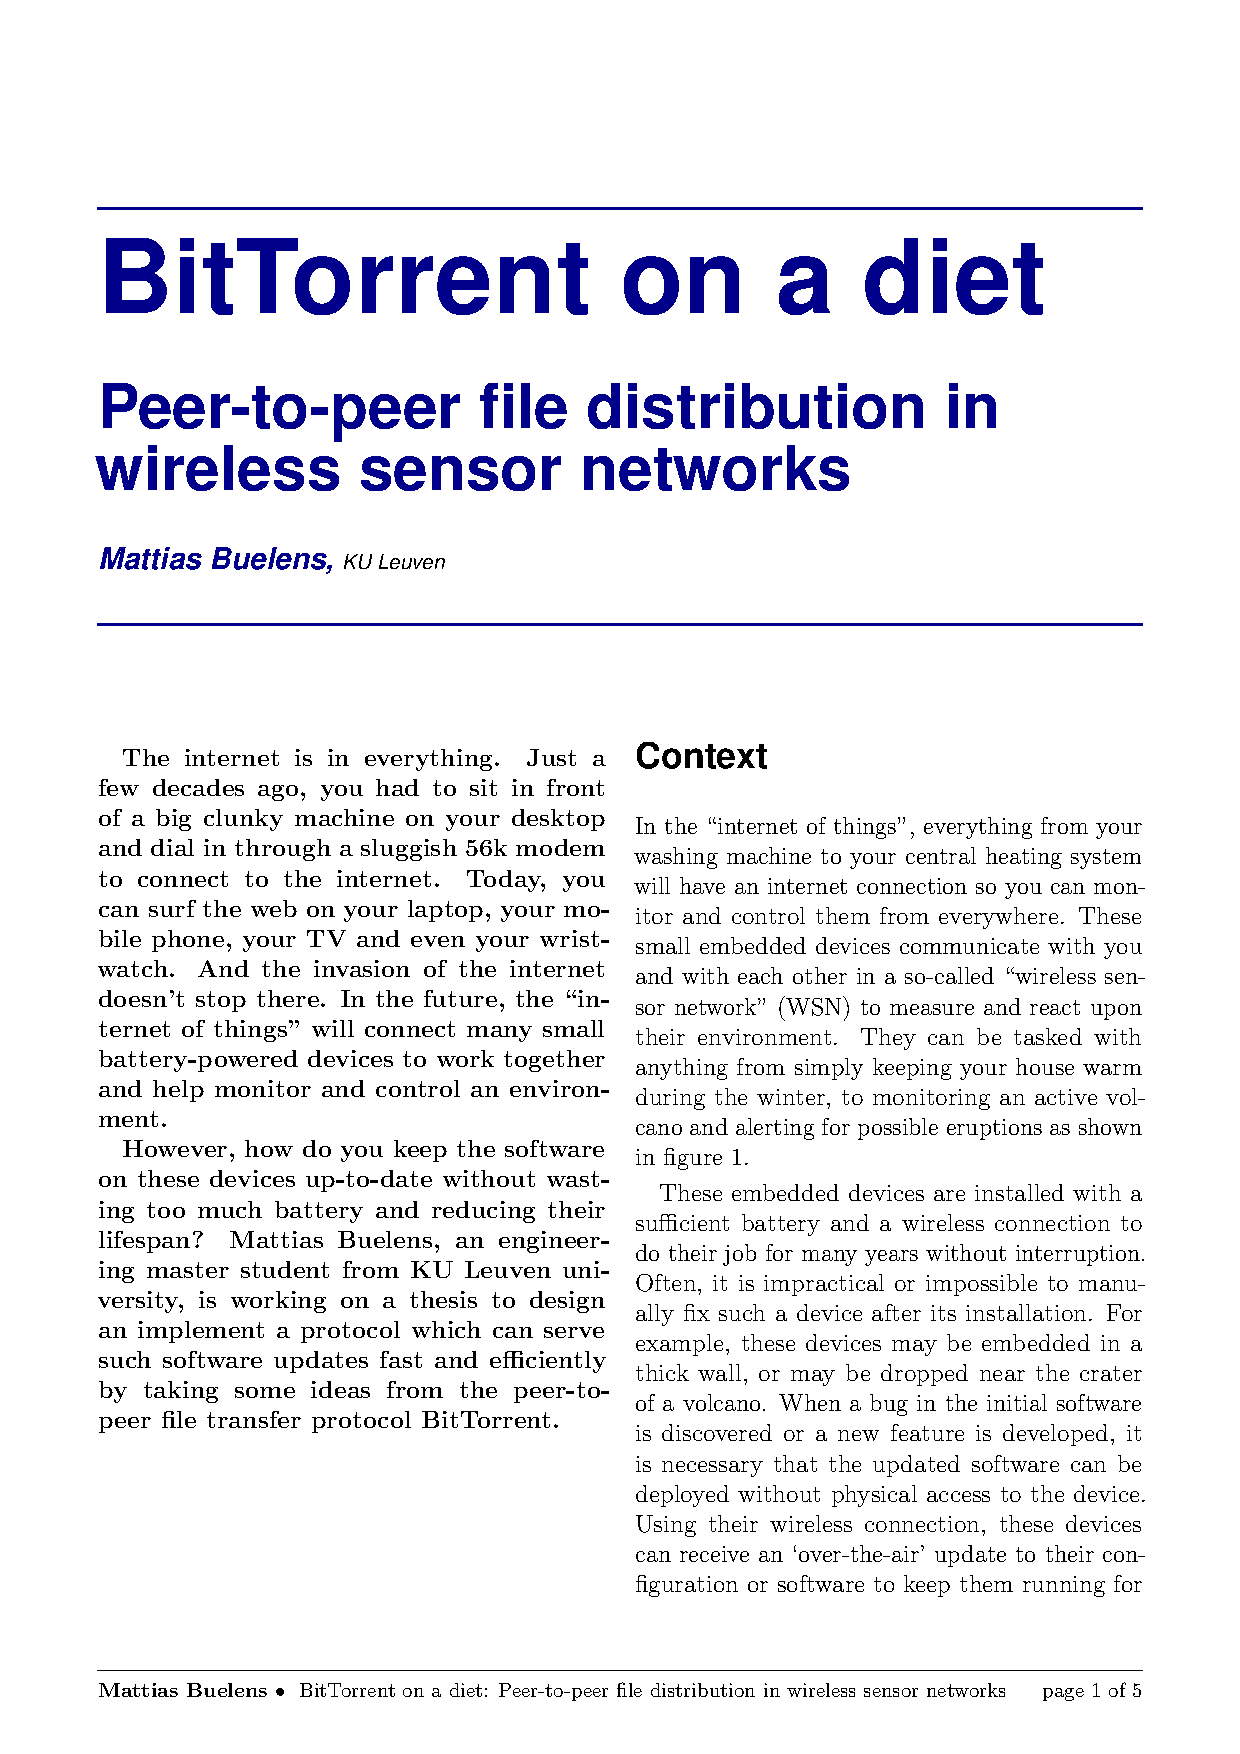
\includepdf[pages=-]{popular-article.pdf}
\chapter{IEEE article (Dutch)}
\label{app:ieee}

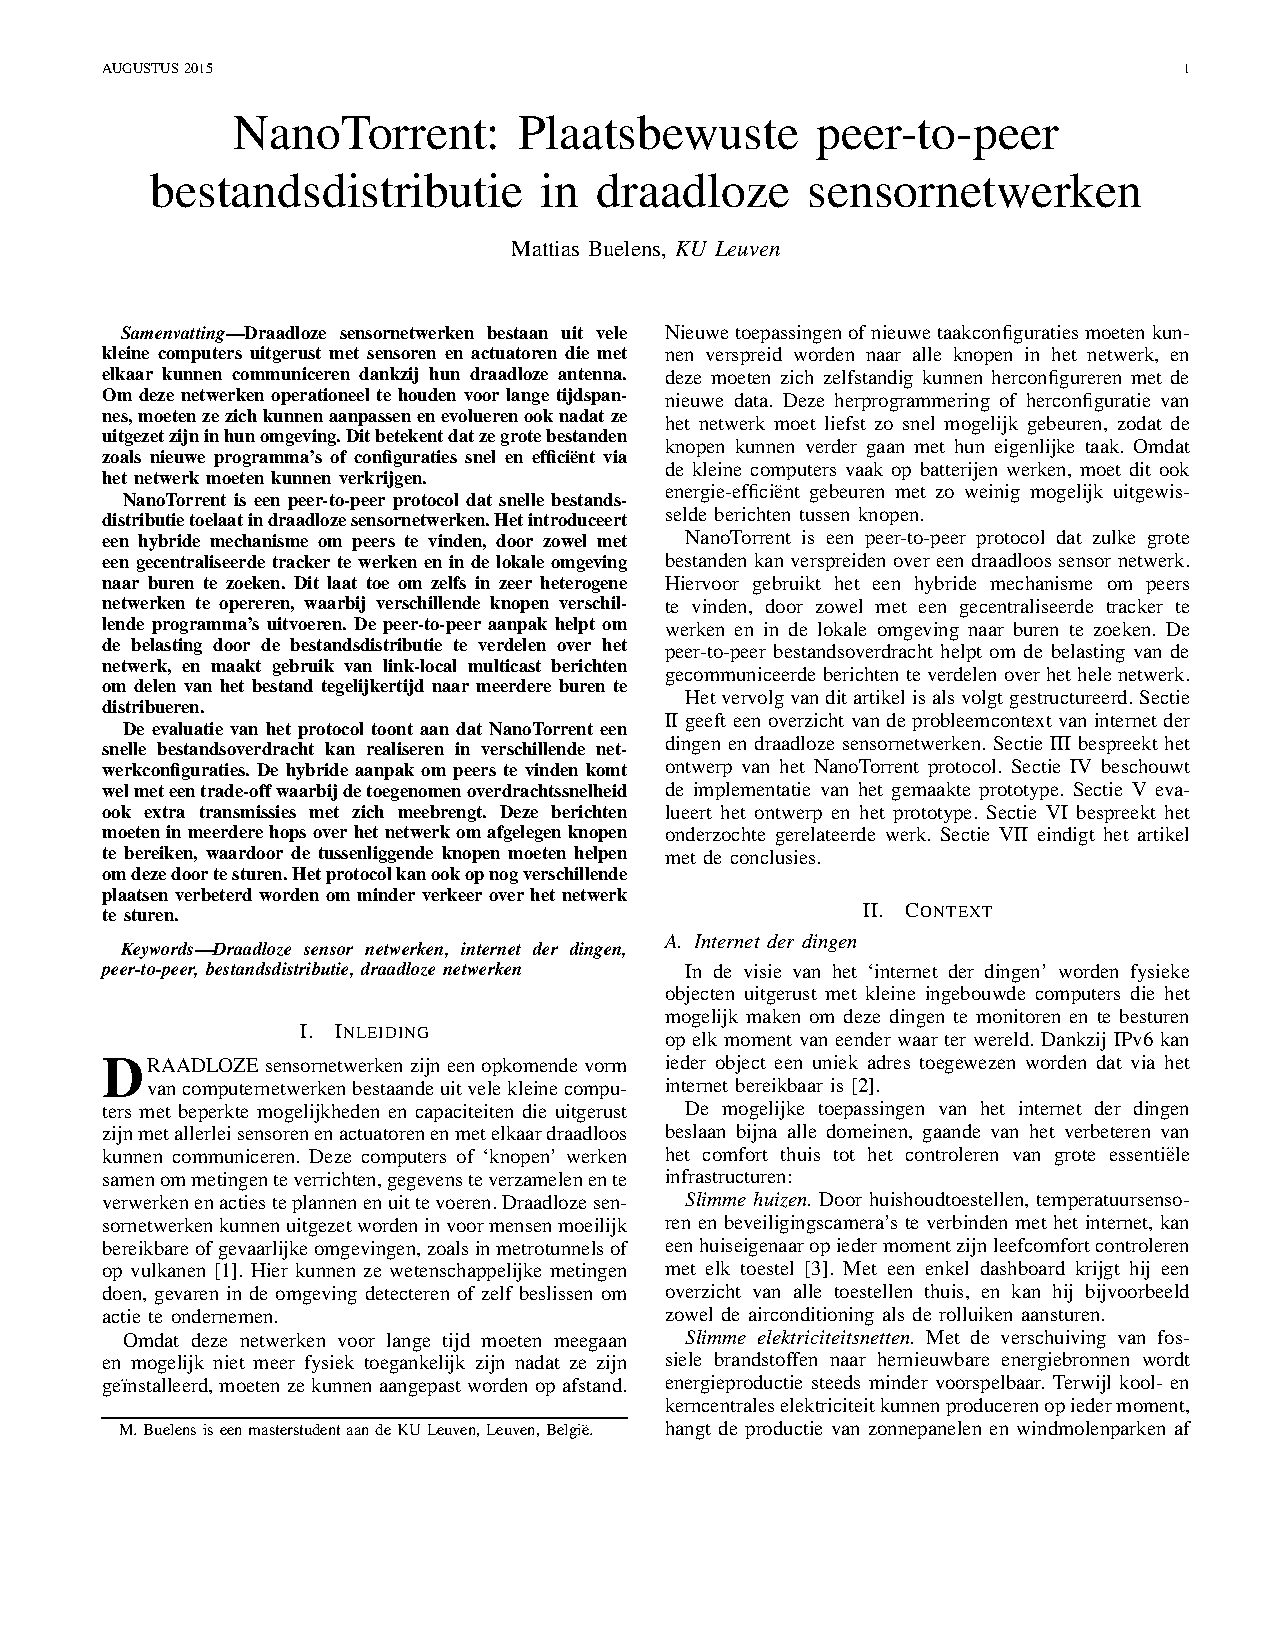
\includepdf[pages=-]{ieee-article.pdf}

\backmatter
% The bibliography comes after the appendices.
% You can replace the standard "abbrv" bibliography style by another one.
\bibliographystyle{plain}
\bibliography{references}

\end{document}
